\documentclass[12pt,]{article}
\usepackage{lmodern}
\usepackage{amssymb,amsmath}
\usepackage{ifxetex,ifluatex}
\usepackage{fixltx2e} % provides \textsubscript
\ifnum 0\ifxetex 1\fi\ifluatex 1\fi=0 % if pdftex
  \usepackage[T1]{fontenc}
  \usepackage[utf8]{inputenc}
\else % if luatex or xelatex
  \ifxetex
    \usepackage{mathspec}
  \else
    \usepackage{fontspec}
  \fi
  \defaultfontfeatures{Ligatures=TeX,Scale=MatchLowercase}
    \setmainfont[]{Times New Roman}
\fi
% use upquote if available, for straight quotes in verbatim environments
\IfFileExists{upquote.sty}{\usepackage{upquote}}{}
% use microtype if available
\IfFileExists{microtype.sty}{%
\usepackage{microtype}
\UseMicrotypeSet[protrusion]{basicmath} % disable protrusion for tt fonts
}{}
\usepackage[margin=2.54cm]{geometry}
\usepackage{hyperref}
\hypersetup{unicode=true,
            pdftitle={Covid-19 Trend Analysis and Visualization},
            pdfauthor={Xueying Feng},
            pdfborder={0 0 0},
            breaklinks=true}
\urlstyle{same}  % don't use monospace font for urls
\usepackage{color}
\usepackage{fancyvrb}
\newcommand{\VerbBar}{|}
\newcommand{\VERB}{\Verb[commandchars=\\\{\}]}
\DefineVerbatimEnvironment{Highlighting}{Verbatim}{commandchars=\\\{\}}
% Add ',fontsize=\small' for more characters per line
\usepackage{framed}
\definecolor{shadecolor}{RGB}{248,248,248}
\newenvironment{Shaded}{\begin{snugshade}}{\end{snugshade}}
\newcommand{\AlertTok}[1]{\textcolor[rgb]{0.94,0.16,0.16}{#1}}
\newcommand{\AnnotationTok}[1]{\textcolor[rgb]{0.56,0.35,0.01}{\textbf{\textit{#1}}}}
\newcommand{\AttributeTok}[1]{\textcolor[rgb]{0.77,0.63,0.00}{#1}}
\newcommand{\BaseNTok}[1]{\textcolor[rgb]{0.00,0.00,0.81}{#1}}
\newcommand{\BuiltInTok}[1]{#1}
\newcommand{\CharTok}[1]{\textcolor[rgb]{0.31,0.60,0.02}{#1}}
\newcommand{\CommentTok}[1]{\textcolor[rgb]{0.56,0.35,0.01}{\textit{#1}}}
\newcommand{\CommentVarTok}[1]{\textcolor[rgb]{0.56,0.35,0.01}{\textbf{\textit{#1}}}}
\newcommand{\ConstantTok}[1]{\textcolor[rgb]{0.00,0.00,0.00}{#1}}
\newcommand{\ControlFlowTok}[1]{\textcolor[rgb]{0.13,0.29,0.53}{\textbf{#1}}}
\newcommand{\DataTypeTok}[1]{\textcolor[rgb]{0.13,0.29,0.53}{#1}}
\newcommand{\DecValTok}[1]{\textcolor[rgb]{0.00,0.00,0.81}{#1}}
\newcommand{\DocumentationTok}[1]{\textcolor[rgb]{0.56,0.35,0.01}{\textbf{\textit{#1}}}}
\newcommand{\ErrorTok}[1]{\textcolor[rgb]{0.64,0.00,0.00}{\textbf{#1}}}
\newcommand{\ExtensionTok}[1]{#1}
\newcommand{\FloatTok}[1]{\textcolor[rgb]{0.00,0.00,0.81}{#1}}
\newcommand{\FunctionTok}[1]{\textcolor[rgb]{0.00,0.00,0.00}{#1}}
\newcommand{\ImportTok}[1]{#1}
\newcommand{\InformationTok}[1]{\textcolor[rgb]{0.56,0.35,0.01}{\textbf{\textit{#1}}}}
\newcommand{\KeywordTok}[1]{\textcolor[rgb]{0.13,0.29,0.53}{\textbf{#1}}}
\newcommand{\NormalTok}[1]{#1}
\newcommand{\OperatorTok}[1]{\textcolor[rgb]{0.81,0.36,0.00}{\textbf{#1}}}
\newcommand{\OtherTok}[1]{\textcolor[rgb]{0.56,0.35,0.01}{#1}}
\newcommand{\PreprocessorTok}[1]{\textcolor[rgb]{0.56,0.35,0.01}{\textit{#1}}}
\newcommand{\RegionMarkerTok}[1]{#1}
\newcommand{\SpecialCharTok}[1]{\textcolor[rgb]{0.00,0.00,0.00}{#1}}
\newcommand{\SpecialStringTok}[1]{\textcolor[rgb]{0.31,0.60,0.02}{#1}}
\newcommand{\StringTok}[1]{\textcolor[rgb]{0.31,0.60,0.02}{#1}}
\newcommand{\VariableTok}[1]{\textcolor[rgb]{0.00,0.00,0.00}{#1}}
\newcommand{\VerbatimStringTok}[1]{\textcolor[rgb]{0.31,0.60,0.02}{#1}}
\newcommand{\WarningTok}[1]{\textcolor[rgb]{0.56,0.35,0.01}{\textbf{\textit{#1}}}}
\usepackage{longtable,booktabs}
\usepackage{graphicx,grffile}
\makeatletter
\def\maxwidth{\ifdim\Gin@nat@width>\linewidth\linewidth\else\Gin@nat@width\fi}
\def\maxheight{\ifdim\Gin@nat@height>\textheight\textheight\else\Gin@nat@height\fi}
\makeatother
% Scale images if necessary, so that they will not overflow the page
% margins by default, and it is still possible to overwrite the defaults
% using explicit options in \includegraphics[width, height, ...]{}
\setkeys{Gin}{width=\maxwidth,height=\maxheight,keepaspectratio}
\IfFileExists{parskip.sty}{%
\usepackage{parskip}
}{% else
\setlength{\parindent}{0pt}
\setlength{\parskip}{6pt plus 2pt minus 1pt}
}
\setlength{\emergencystretch}{3em}  % prevent overfull lines
\providecommand{\tightlist}{%
  \setlength{\itemsep}{0pt}\setlength{\parskip}{0pt}}
\setcounter{secnumdepth}{5}
% Redefines (sub)paragraphs to behave more like sections
\ifx\paragraph\undefined\else
\let\oldparagraph\paragraph
\renewcommand{\paragraph}[1]{\oldparagraph{#1}\mbox{}}
\fi
\ifx\subparagraph\undefined\else
\let\oldsubparagraph\subparagraph
\renewcommand{\subparagraph}[1]{\oldsubparagraph{#1}\mbox{}}
\fi

%%% Use protect on footnotes to avoid problems with footnotes in titles
\let\rmarkdownfootnote\footnote%
\def\footnote{\protect\rmarkdownfootnote}

%%% Change title format to be more compact
\usepackage{titling}

% Create subtitle command for use in maketitle
\providecommand{\subtitle}[1]{
  \posttitle{
    \begin{center}\large#1\end{center}
    }
}

\setlength{\droptitle}{-2em}

  \title{Covid-19 Trend Analysis and Visualization}
    \pretitle{\vspace{\droptitle}\centering\huge}
  \posttitle{\par}
  \subtitle{\url{https://github.com/xueying-F/ENV872-Project_XY_Feng}}
  \author{Xueying Feng}
    \preauthor{\centering\large\emph}
  \postauthor{\par}
    \date{}
    \predate{}\postdate{}
  

\begin{document}
\maketitle

\newpage
\tableofcontents 
\newpage
\listoftables 
\newpage
\listoffigures 
\newpage

\hypertarget{rationale-and-research-questions}{%
\section{Rationale and Research
Questions}\label{rationale-and-research-questions}}

China broke out a global disease, COVID-19, in December 2019. It has
been confirmed that it is a new type of virus called 2019 new
coronavirus (2019-nCoV) in Jan 2020. The World Health Organization (WHO)
announced the official new name of the disease caused by nCoV2019 (2019
novel coronavirus) in Feb 2020. The CDC noted that the symptoms of the
new coronavirus include "symptoms of fever and lower respiratory tract
disease (eg. coughing, difficulty breathing). There is currently no
vaccine, and because this is a virus, antibiotics will not work.

COVID-19 has spread worldwide in just four months, and more than 2.7
million people have been sick. It is a global pandemic disease announced
by the World Health Organization (WHO). Also, it can easily infect
humans, and can spread from person to person in a rapid and sustained
manner. This research focus on the datasets from China, United States,
and whole global countries to see the trend of confirmed cases, death
cases and heal cases. Moreover, I will combine some news and report into
policies in each country to analyze the trend patterns.

The research question is:\\
(1) Is there a same trend pattern on China and United States?\\
(2) What is trend pattern on global level?\\
(3) Why trend patterns look like that?

Downloading datasets from R package, nCov2019
(\url{https://github.com/GuangchuangYu/nCov2019}), which provides
convenient access to epidemiological data on the coronavirus outbreak,
which contains real-time data and historical data for each country.
Please see the detail information in Dataset Information setion.

\newpage

\hypertarget{dataset-information}{%
\section{Dataset Information}\label{dataset-information}}

\hypertarget{database-information}{%
\subsection{Database Information}\label{database-information}}

I access all Novel Coronavirus data from the R package, nCov2019, which
includes detailed real-time statistics, historical data in all
countries, and down to the city-level.

More information can be found
here:\url{https://github.com/GuangchuangYu/nCov2019}.

\hypertarget{data-content-information}{%
\subsection{Data Content Information}\label{data-content-information}}

I pulled all relevent data from nCov2019 package. I named all pulled
data as raw.csv and then saved into Data/Raw folder. Beside, I wrangled
all raw and selected the relevent columns, and then saved into
Data/Processed folder. Because data pulled from nCov2019 package are
real-time data, I kept the update time on April 16th, 2020. Therefore,
the following descriptions of my datasets are for processed data.

\begin{longtable}[]{@{}cc@{}}
\caption{Historical\_Global\_processed dataset}\tabularnewline
\toprule
Column name & Description\tabularnewline
\midrule
\endfirsthead
\toprule
Column name & Description\tabularnewline
\midrule
\endhead
time & Date\tabularnewline
country & Country name\tabularnewline
cum\_confirm & Cumulative number of COVID-19 confirmed
cases\tabularnewline
cum\_heal & Cumulative number of COVID-19 heal cases\tabularnewline
cum\_dead & Cumulative number of COVID-19 death cases\tabularnewline
\bottomrule
\end{longtable}

\begin{longtable}[]{@{}cc@{}}
\caption{Historical\_China\_processed dataset}\tabularnewline
\toprule
Column name & Description\tabularnewline
\midrule
\endfirsthead
\toprule
Column name & Description\tabularnewline
\midrule
\endhead
time & Date\tabularnewline
country & Country name\tabularnewline
province & Province name\tabularnewline
city & City name\tabularnewline
cum\_confirm & Cumulative number of COVID-19 confirmed
cases\tabularnewline
cum\_heal & Cumulative number of COVID-19 heal cases\tabularnewline
cum\_dead & Cumulative number of COVID-19 death cases\tabularnewline
\bottomrule
\end{longtable}

\begin{longtable}[]{@{}cc@{}}
\caption{Covid19\_Global\_processed dataset}\tabularnewline
\toprule
Column name & Description\tabularnewline
\midrule
\endfirsthead
\toprule
Column name & Description\tabularnewline
\midrule
\endhead
name & Country name\tabularnewline
confirm & Number of COVID-19 confirmed cases\tabularnewline
dead & Number of COVID-19 death cases\tabularnewline
deadRate & Total death number/ Cumulative total number of COVID-19
cases(\%)\tabularnewline
heal & number of COVID-19 heal cases\tabularnewline
healRate & Total heal number/ Cumulative total number of COVID-19
cases(\%)\tabularnewline
\bottomrule
\end{longtable}

\begin{longtable}[]{@{}cc@{}}
\caption{Covid19\_China\_processed dataset}\tabularnewline
\toprule
Column name & Description\tabularnewline
\midrule
\endfirsthead
\toprule
Column name & Description\tabularnewline
\midrule
\endhead
name & Province name\tabularnewline
confirm & Number of COVID-19 confirmed cases\tabularnewline
dead & Number of COVID-19 death cases\tabularnewline
deadRate & Total death number/ Cumulative total number of COVID-19
cases(\%)\tabularnewline
heal & number of COVID-19 heal cases\tabularnewline
healRate & Total heal number/ Cumulative total number of COVID-19
cases(\%)\tabularnewline
\bottomrule
\end{longtable}

\begin{longtable}[]{@{}ccc@{}}
\caption{Covid19\_US\_processed dataset}\tabularnewline
\toprule
Column name & Description & NA\tabularnewline
\midrule
\endfirsthead
\toprule
Column name & Description & NA\tabularnewline
\midrule
\endhead
time & Date & NA\tabularnewline
country & United States & NA\tabularnewline
province & States name & NA\tabularnewline
cum\_confirm & Cumulative number of COVID-19 confirmed cases &
NA\tabularnewline
cum\_heal & Cumulative number of COVID-19 heal cases & NA\tabularnewline
cum\_dead & Cumulative number of COVID-19 death cases &
NA\tabularnewline
\bottomrule
\end{longtable}

\newpage

\hypertarget{exploratory-analysis}{%
\section{Exploratory Analysis}\label{exploratory-analysis}}

Wrangling the raw data for thess datasets is to select the columns that
are useful for this research. After wrangling all dataset, they are
saved into processed folder. However, this section will show how
processed data form, but processed data will be directly used to do
analysis. During analysis, datasets will be wrangled again based on
anlysis requirments.

\begin{Shaded}
\begin{Highlighting}[]
\CommentTok{#Covid19_China_raw <- read.csv("Covid19_China_raw.csv",}
\CommentTok{#                     header=TRUE,stringsAsFactors = FALSE, strip.white = TRUE,sep = ',')}
\CommentTok{#Covid19_China_processed <- }
\CommentTok{#  select(Covid19_China_raw, name, confirm, dead, deadRate, heal, healRate)}


\CommentTok{#Covid19_US_raw <- read.csv("Covid19_US_raw.csv", header=TRUE,}
\CommentTok{#                  stringsAsFactors = FALSE, strip.white = TRUE,sep = ',')}
\CommentTok{#Covid19_US_processed <- }
\CommentTok{#  select(Covid19_US_raw, time:cum_dead)}


\CommentTok{#Covid19_Global_raw <- read.csv("Covid19_Global_raw.csv",}
\CommentTok{#                      header=TRUE,stringsAsFactors = FALSE, strip.white = TRUE,sep = ',')}
\CommentTok{#Covid19_Global_processed <- }
\CommentTok{#  select(Covid19_Global_raw, name, confirm, dead, deadRate,heal, healRate)}


\CommentTok{#historical_China_raw <- read.csv("historical_China_raw.csv",}
\CommentTok{#                        header=TRUE,stringsAsFactors = FALSE, strip.white = TRUE,sep = ',')}
\CommentTok{#Historical_China_processed <- }
\CommentTok{#  select(historical_China_raw, time:cum_dead)}


\CommentTok{#historical_Global_raw <- read.csv("historical_Global_raw.csv", header=TRUE, }
\CommentTok{#                                  stringsAsFactors = FALSE, strip.white = TRUE,sep = ',')}
\CommentTok{#Historical_Global_processed <- historical_Global_raw}
\end{Highlighting}
\end{Shaded}

\hypertarget{explore-china-dataset}{%
\subsection{Explore China Dataset}\label{explore-china-dataset}}

\begin{Shaded}
\begin{Highlighting}[]
\NormalTok{Covid19_China_processed <-}\StringTok{ }\KeywordTok{read.csv}\NormalTok{(}\StringTok{"./Data/Processed/Covid19_China_processed.csv"}\NormalTok{)}

\CommentTok{# Check data frame}
\KeywordTok{colnames}\NormalTok{(Covid19_China_processed)}
\KeywordTok{head}\NormalTok{(Covid19_China_processed)}
\end{Highlighting}
\end{Shaded}

\begin{Shaded}
\begin{Highlighting}[]
\CommentTok{# scale_y_log10: transform the y-axis to make it easier to read}
\NormalTok{China.plot <-}\KeywordTok{ggplot}\NormalTok{(Covid19_China_processed,}\KeywordTok{aes}\NormalTok{(}\DataTypeTok{x =}\NormalTok{ name,}\DataTypeTok{y =}\NormalTok{ confirm)) }\OperatorTok{+}\StringTok{ }
\StringTok{  }\KeywordTok{geom_bar}\NormalTok{(}\DataTypeTok{size =} \DecValTok{2}\NormalTok{, }\DataTypeTok{stat =} \StringTok{"identity"}\NormalTok{,}\DataTypeTok{position =} \StringTok{"dodge"}\NormalTok{, }\DataTypeTok{fill =}\StringTok{"#fdae6b"}\NormalTok{) }\OperatorTok{+}\StringTok{ }
\StringTok{  }\KeywordTok{scale_y_log10}\NormalTok{() }\OperatorTok{+}
\StringTok{  }\KeywordTok{labs}\NormalTok{(}\DataTypeTok{x=} \StringTok{"Province Name (China)"}\NormalTok{,}
       \DataTypeTok{y =} \StringTok{"Numbers of Confirmed Cases"}\NormalTok{) }\OperatorTok{+}\StringTok{ }
\StringTok{  }\NormalTok{mytheme }\OperatorTok{+}
\StringTok{  }\KeywordTok{theme}\NormalTok{(}\DataTypeTok{axis.text.x =} \KeywordTok{element_text}\NormalTok{(}\DataTypeTok{angle =} \DecValTok{45}\NormalTok{, }\DataTypeTok{hjust =} \DecValTok{1}\NormalTok{))}

\KeywordTok{print}\NormalTok{(China.plot)}
\end{Highlighting}
\end{Shaded}

\begin{figure}
\centering
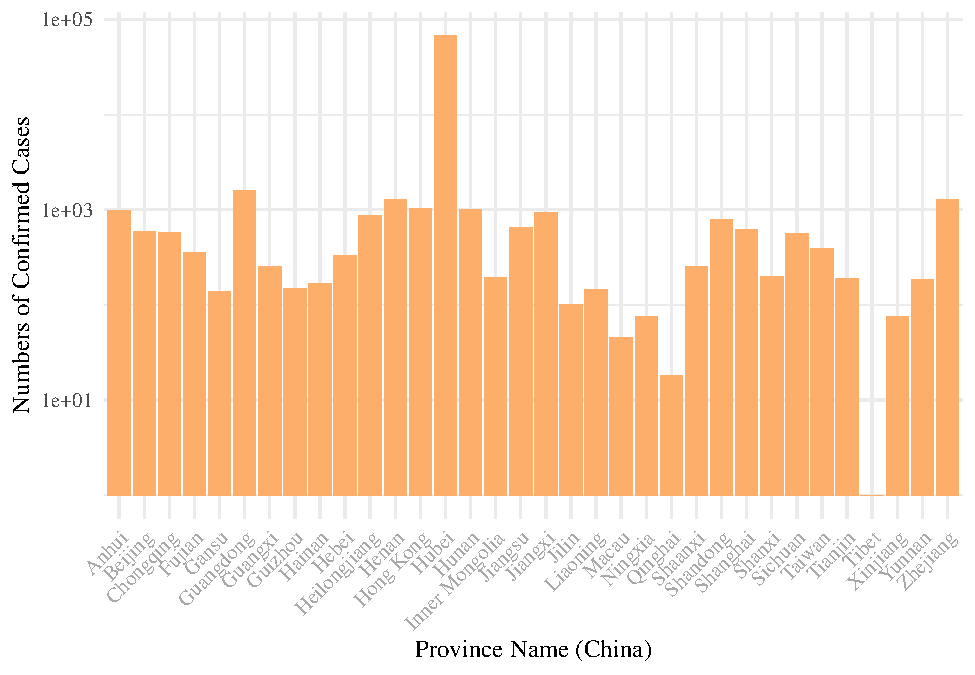
\includegraphics{Feng_ENV872_Project_files/figure-latex/China.plot-1.pdf}
\caption{Compare total confimed number in each province in China}
\end{figure}

\hypertarget{explore-global-dataset}{%
\subsection{Explore Global Dataset}\label{explore-global-dataset}}

\textbf{Top 15 countries}

\begin{Shaded}
\begin{Highlighting}[]
\NormalTok{Covid19_Global_processed <-}\StringTok{ }\KeywordTok{read.csv}\NormalTok{(}\StringTok{"./Data/Processed/Covid19_Global_processed.csv"}\NormalTok{)}

\CommentTok{# Check data frame}
\KeywordTok{head}\NormalTok{(Historical_Global_processed)}
\KeywordTok{str}\NormalTok{(Historical_Global_processed)}

\CommentTok{# Change date column to date}
\NormalTok{Historical_Global_processed}\OperatorTok{$}\NormalTok{time <-}\StringTok{ }\KeywordTok{as.Date}\NormalTok{(Historical_Global_processed}\OperatorTok{$}\NormalTok{time, }
                                            \DataTypeTok{format =} \StringTok{"%Y-%m-%d"}\NormalTok{) }
\KeywordTok{class}\NormalTok{(Historical_Global_processed}\OperatorTok{$}\NormalTok{time)}


\CommentTok{# Filter out top 15 countries with the highest number of diagnoses}
\NormalTok{Fifty_countries <-}\StringTok{ }\NormalTok{Covid19_Global_processed }\OperatorTok\StringTok{ }
\StringTok{  }\KeywordTok{top_n}\NormalTok{(}\DecValTok{15}\NormalTok{, confirm) }\OperatorTok
\StringTok{  }\KeywordTok{arrange}\NormalTok{(}\KeywordTok{desc}\NormalTok{(confirm))}

\CommentTok{# Save as csv}
\KeywordTok{write.csv}\NormalTok{(Fifty_countries,}
          \DataTypeTok{file =} \StringTok{"./Data/Processed/Top_Fifty_countries (cum).csv"}\NormalTok{, }\DataTypeTok{row.names=}\OtherTok{FALSE}\NormalTok{)}
\end{Highlighting}
\end{Shaded}

\begin{Shaded}
\begin{Highlighting}[]
\CommentTok{# Draw histogram plot}
\NormalTok{Global.plot <-}\KeywordTok{ggplot}\NormalTok{(Fifty_countries,}\KeywordTok{aes}\NormalTok{(}\DataTypeTok{x =}\NormalTok{ name,}\DataTypeTok{y =}\NormalTok{ confirm)) }\OperatorTok{+}\StringTok{ }
\StringTok{  }\KeywordTok{geom_bar}\NormalTok{(}\DataTypeTok{size =} \DecValTok{2}\NormalTok{, }\DataTypeTok{stat =} \StringTok{"identity"}\NormalTok{,}\DataTypeTok{position =} \StringTok{"dodge"}\NormalTok{, }\DataTypeTok{fill =}\StringTok{"#fdae6b"}\NormalTok{) }\OperatorTok{+}\StringTok{ }
\StringTok{  }\KeywordTok{labs}\NormalTok{(}\DataTypeTok{x =} \StringTok{" Country Name (Top 15)"}\NormalTok{,}
       \DataTypeTok{y =} \StringTok{"Numbers of Confirmed Cases"}\NormalTok{) }\OperatorTok{+}\StringTok{ }
\StringTok{  }\NormalTok{mytheme }\OperatorTok{+}
\StringTok{  }\KeywordTok{theme}\NormalTok{(}\DataTypeTok{axis.text.x =} \KeywordTok{element_text}\NormalTok{(}\DataTypeTok{angle =} \DecValTok{45}\NormalTok{, }\DataTypeTok{hjust =} \DecValTok{1}\NormalTok{))}

\KeywordTok{print}\NormalTok{(Global.plot)}
\end{Highlighting}
\end{Shaded}

\begin{figure}
\centering
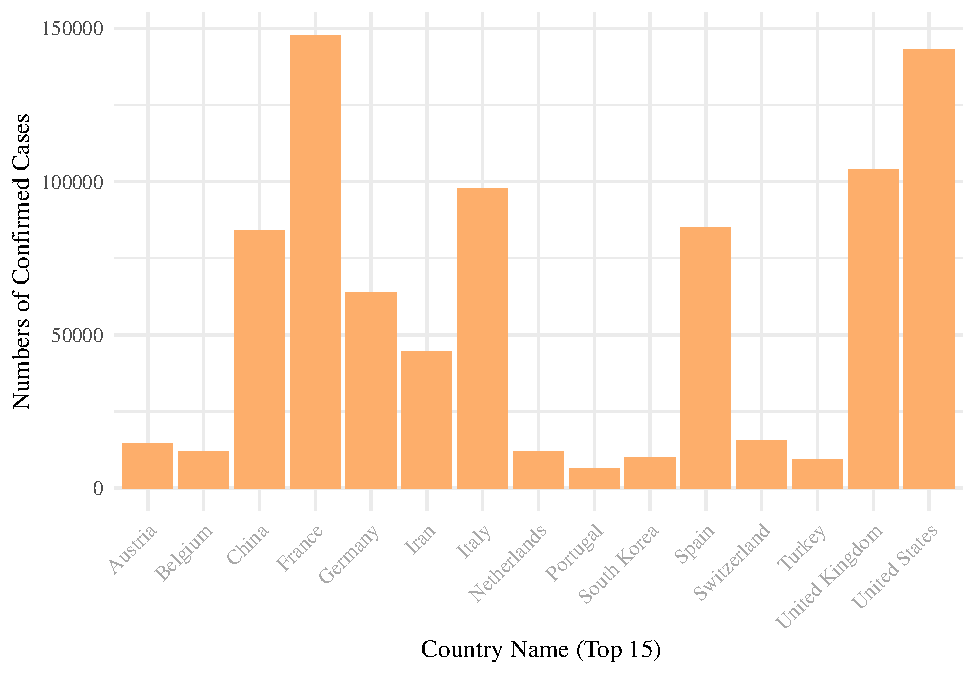
\includegraphics{Feng_ENV872_Project_files/figure-latex/Global.plot-1.pdf}
\caption{Compare total confimed number of each country}
\end{figure}

\hypertarget{explore-united-states-dataset}{%
\subsection{Explore United States
Dataset}\label{explore-united-states-dataset}}

\textbf{Map of comfimed cases distribution in United State}

\begin{Shaded}
\begin{Highlighting}[]
\CommentTok{# Check data}
\KeywordTok{head}\NormalTok{(Covid19_US_processed)}
\KeywordTok{str}\NormalTok{(Covid19_US_processed)}

\CommentTok{# Change date column to date}
\NormalTok{Covid19_US_processed}\OperatorTok{$}\NormalTok{time <-}\StringTok{ }\KeywordTok{as.Date}\NormalTok{(Covid19_US_processed}\OperatorTok{$}\NormalTok{time, }\DataTypeTok{format =} \StringTok{"%m/%d/%y"}\NormalTok{) }
\KeywordTok{class}\NormalTok{(Covid19_US_processed}\OperatorTok{$}\NormalTok{time)}

\CommentTok{# Check column names}
\KeywordTok{colnames}\NormalTok{(Covid19_US_processed)}

\CommentTok{# Rename column where names is "province"}
\KeywordTok{names}\NormalTok{(Covid19_US_processed)[}\KeywordTok{names}\NormalTok{(Covid19_US_processed) }\OperatorTok{==}\StringTok{ "province"}\NormalTok{] <-}\StringTok{ "state"}
\KeywordTok{str}\NormalTok{(Covid19_US_processed)}


\CommentTok{# Select total confirmed cases in 51 States}
\NormalTok{US_States <-}\StringTok{ }\NormalTok{Covid19_US_processed }\OperatorTok
\StringTok{  }\KeywordTok{filter}\NormalTok{(time }\OperatorTok{==}\StringTok{ }\KeywordTok{as.Date}\NormalTok{(}\StringTok{"2020-04-16"}\NormalTok{)) }\OperatorTok
\StringTok{  }\KeywordTok{filter}\NormalTok{(state}\OperatorTok{!=}\StringTok{ "Unpublished sources"}\NormalTok{) }\OperatorTok
\StringTok{  }\KeywordTok{top_n}\NormalTok{(}\DecValTok{51}\NormalTok{, cum_confirm)}

\CommentTok{# Convert state column to characters }
\NormalTok{US_States}\OperatorTok{$}\NormalTok{state <-}\StringTok{ }\KeywordTok{as.character}\NormalTok{(US_States}\OperatorTok{$}\NormalTok{state)}

\CommentTok{# Rename specific cell name}
\NormalTok{US_States}\OperatorTok{$}\NormalTok{state[US_States}\OperatorTok{$}\NormalTok{state }\OperatorTok{==}\StringTok{ 'New York state'}\NormalTok{] <-}\StringTok{ 'New York'}
\NormalTok{US_States}\OperatorTok{$}\NormalTok{state[US_States}\OperatorTok{$}\NormalTok{state }\OperatorTok{==}\StringTok{ "Washington State"}\NormalTok{] <-}\StringTok{ "Washington"}
\NormalTok{US_States}\OperatorTok{$}\NormalTok{state[US_States}\OperatorTok{$}\NormalTok{state }\OperatorTok{==}\StringTok{ 'the state of Wisconsin'}\NormalTok{] <-}\StringTok{ 'Wisconsin'}
\end{Highlighting}
\end{Shaded}

\begin{Shaded}
\begin{Highlighting}[]
\CommentTok{#install.packages("usmap")}
\KeywordTok{library}\NormalTok{(usmap)}

\NormalTok{USMap_Base <-}\StringTok{ }\KeywordTok{plot_usmap}\NormalTok{(}\DataTypeTok{regions =} \StringTok{"counties"}\NormalTok{) }\OperatorTok{+}\StringTok{ }
\StringTok{  }\KeywordTok{labs}\NormalTok{(}\DataTypeTok{title =} \StringTok{"US Counties"}\NormalTok{,}
       \DataTypeTok{subtitle =} \StringTok{"This is a blank map of the counties of the United States."}\NormalTok{) }\OperatorTok{+}\StringTok{ }
\StringTok{  }\KeywordTok{theme}\NormalTok{(}\DataTypeTok{panel.background =} \KeywordTok{element_rect}\NormalTok{(}\DataTypeTok{color =} \StringTok{"black"}\NormalTok{, }\DataTypeTok{fill =} \StringTok{"lightblue"}\NormalTok{))}


\CommentTok{### Draw US Case distribution on map}
\NormalTok{US.map <-}\StringTok{ }\KeywordTok{plot_usmap}\NormalTok{(}\DataTypeTok{regions=}\StringTok{"state"}\NormalTok{, }\DataTypeTok{data =}\NormalTok{ US_States, }
                                \DataTypeTok{values =} \StringTok{"cum_confirm"}\NormalTok{, }\DataTypeTok{color =} \StringTok{"black"}\NormalTok{) }\OperatorTok{+}
\StringTok{  }\KeywordTok{scale_fill_continuous}\NormalTok{(}\DataTypeTok{low =} \StringTok{"#fee6ce"}\NormalTok{, }\DataTypeTok{high =} \StringTok{"#d95f0e"}\NormalTok{, }
                        \DataTypeTok{name =} \StringTok{"Total confirmed cases"}\NormalTok{, }\DataTypeTok{label =}\NormalTok{ scales}\OperatorTok{::}\NormalTok{comma) }\OperatorTok{+}\StringTok{ }
\StringTok{  }\KeywordTok{labs}\NormalTok{(}\DataTypeTok{title =} \StringTok{"State Reporting Cases of Covid 19"}\NormalTok{) }\OperatorTok{+}
\StringTok{  }\KeywordTok{theme}\NormalTok{(}\DataTypeTok{legend.position =} \StringTok{"right"}\NormalTok{)}

\KeywordTok{print}\NormalTok{(US.map)}
\end{Highlighting}
\end{Shaded}

\begin{figure}
\centering
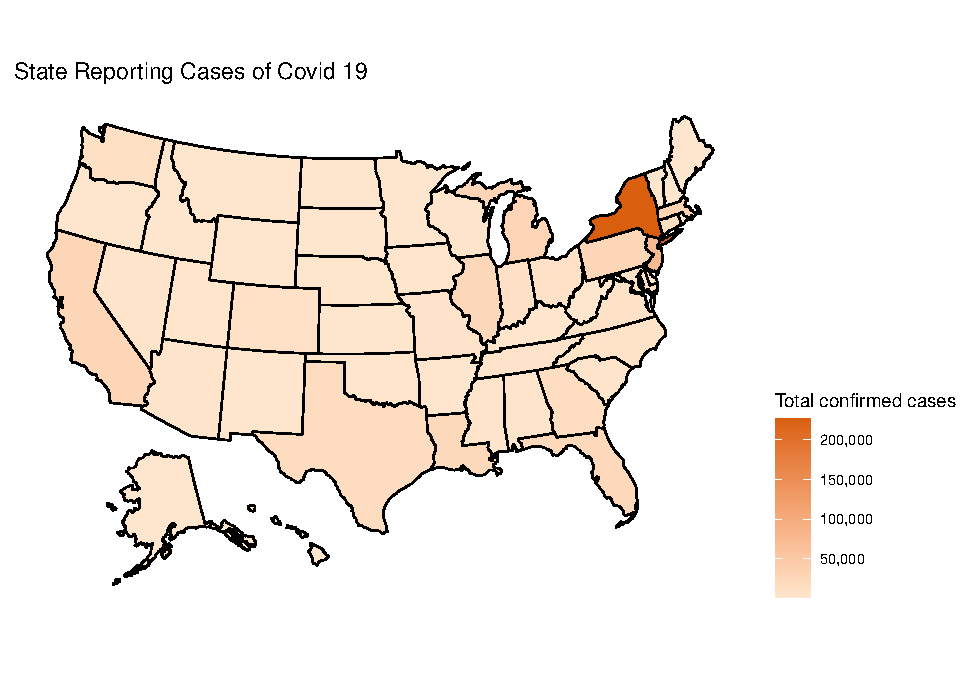
\includegraphics{Feng_ENV872_Project_files/figure-latex/US.map-1.pdf}
\caption{Map of comfimed cases didtribution in United State}
\end{figure}

\begin{quote}
Figure 1 shows the total confimed number of each province in China
(update on April 16th, 2020). Due to this graph, I will seperate Hubei
province and other provinces in China and see their trend patterns.
\end{quote}

\begin{quote}
Figure 2 shows the total confimed number of each country (update on
April 16th, 2020). Due to this graph, I will focus on the United States
dataset and see its trend pattern.
\end{quote}

\begin{quote}
Figure 3 shows confirmed cases distribution in each state by using map,
which can make readers straighter forward to see which states are more
serious.
\end{quote}

\newpage

\hypertarget{analysis}{%
\section{Analysis}\label{analysis}}

\hypertarget{anlysis-trend-of-confirmed-cases-in-china}{%
\subsection{Anlysis trend of confirmed cases in
China}\label{anlysis-trend-of-confirmed-cases-in-china}}

\hypertarget{trend-of-total-confirmed-cases-in-china}{%
\subsubsection{Trend of Total confirmed cases in
China}\label{trend-of-total-confirmed-cases-in-china}}

\begin{Shaded}
\begin{Highlighting}[]
\CommentTok{# Selsct data from China}
\KeywordTok{str}\NormalTok{(Historical_Global_processed)}
\end{Highlighting}
\end{Shaded}

\begin{verbatim}
## 'data.frame':    8687 obs. of  5 variables:
##  $ time       : Date, format: "2019-12-01" "2019-12-02" ...
##  $ country    : Factor w/ 205 levels "Afghanistan",..: 39 39 39 39 39 39 39 39 39 39 ...
##  $ cum_confirm: int  1 1 1 1 1 1 1 1 1 1 ...
##  $ cum_heal   : int  0 0 0 0 0 0 0 0 0 0 ...
##  $ cum_dead   : int  0 0 0 0 0 0 0 0 0 0 ...
\end{verbatim}

\begin{Shaded}
\begin{Highlighting}[]
\NormalTok{Historical_China =}\StringTok{ }\NormalTok{Historical_Global_processed[Historical_Global_processed}\OperatorTok{$}\NormalTok{country }\OperatorTok{==}\StringTok{ 'China'}\NormalTok{,]}
\KeywordTok{head}\NormalTok{(Historical_China)}
\end{Highlighting}
\end{Shaded}

\begin{verbatim}
##         time country cum_confirm cum_heal cum_dead
## 1 2019-12-01   China           1        0        0
## 2 2019-12-02   China           1        0        0
## 3 2019-12-03   China           1        0        0
## 4 2019-12-04   China           1        0        0
## 5 2019-12-05   China           1        0        0
## 6 2019-12-06   China           1        0        0
\end{verbatim}

\begin{Shaded}
\begin{Highlighting}[]
\CommentTok{# Create a ggplot depicting cases incereasing over time}
\NormalTok{China_Total_Trend.plot <-}\StringTok{ }
\StringTok{  }\KeywordTok{ggplot}\NormalTok{(Historical_China, }\KeywordTok{aes}\NormalTok{(}\DataTypeTok{x=}\NormalTok{time, }\DataTypeTok{y=}\NormalTok{cum_confirm)) }\OperatorTok{+}
\StringTok{  }\KeywordTok{geom_point}\NormalTok{(}\DataTypeTok{colour =} \StringTok{"#e6550d"}\NormalTok{) }\OperatorTok{+}
\StringTok{  }\KeywordTok{geom_line}\NormalTok{(}\DataTypeTok{colour =} \StringTok{"#d95f0e"}\NormalTok{) }\OperatorTok{+}
\StringTok{  }\KeywordTok{labs}\NormalTok{(}\DataTypeTok{x =} \StringTok{"Time"}\NormalTok{, }
       \DataTypeTok{y =} \StringTok{"Confirmed Cases"}\NormalTok{) }\OperatorTok{+}\StringTok{ }
\StringTok{  }\KeywordTok{scale_x_date}\NormalTok{(}\DataTypeTok{date_labels =} \StringTok{"%Y-%m-%d"}\NormalTok{)}

\KeywordTok{print}\NormalTok{(China_Total_Trend.plot)}
\end{Highlighting}
\end{Shaded}

\begin{figure}
\centering
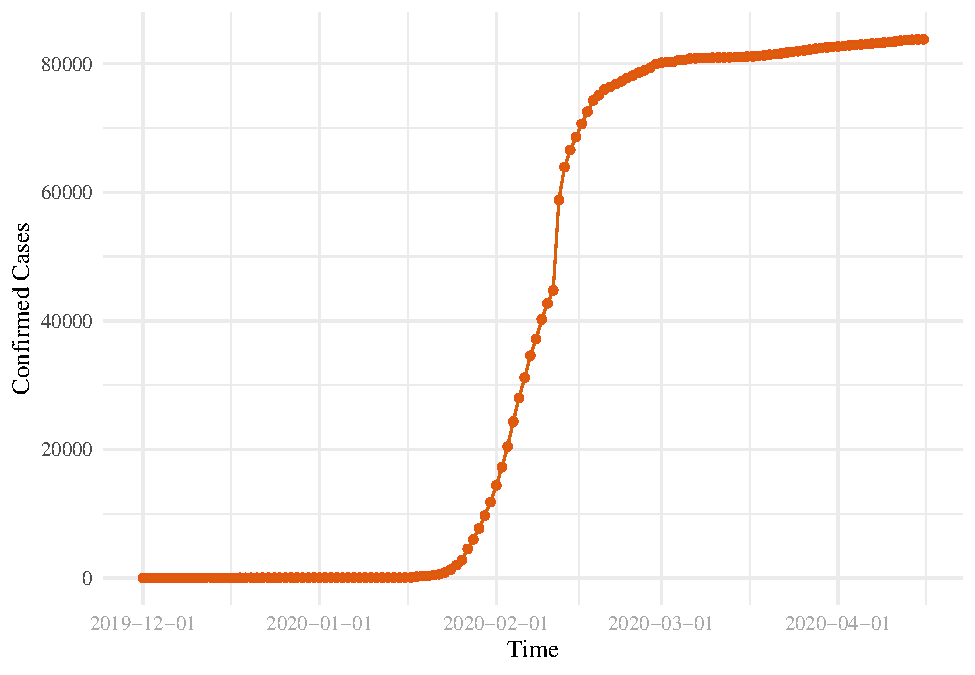
\includegraphics{Feng_ENV872_Project_files/figure-latex/China_Total_Trend.plot-1.pdf}
\caption{Trend of confirmed case in China}
\end{figure}

\hypertarget{trend-of-confirmed-cases-in-each-province-in-china}{%
\subsubsection{Trend of confirmed cases in each province in
China}\label{trend-of-confirmed-cases-in-each-province-in-china}}

\begin{Shaded}
\begin{Highlighting}[]
\CommentTok{# Check data}
\KeywordTok{head}\NormalTok{(Historical_China_processed)}
\KeywordTok{str}\NormalTok{(Historical_China_processed)}

\CommentTok{# Change date column to date}
\NormalTok{Historical_China_processed}\OperatorTok{$}\NormalTok{time <-}\StringTok{ }\KeywordTok{as.Date}\NormalTok{(Historical_China_processed}\OperatorTok{$}\NormalTok{time, }
                                           \DataTypeTok{format =} \StringTok{"%m/%d/%y"}\NormalTok{) }
\KeywordTok{head}\NormalTok{(Historical_China_processed)}
\KeywordTok{class}\NormalTok{(Historical_China_processed}\OperatorTok{$}\NormalTok{time)}
\end{Highlighting}
\end{Shaded}

\hypertarget{trend-of-confirmed-cases-in-hubei-china}{%
\subsubsection{Trend of confirmed cases in Hubei,
China}\label{trend-of-confirmed-cases-in-hubei-china}}

\begin{Shaded}
\begin{Highlighting}[]
\CommentTok{# Select Hubei province data}
\NormalTok{Historical_Hubei =}\StringTok{ }\NormalTok{Historical_China_processed[Historical_China_processed}\OperatorTok{$}\NormalTok{province }\OperatorTok{==}\StringTok{ 'Hubei'}\NormalTok{,]}
\KeywordTok{head}\NormalTok{(Historical_Hubei)}

\CommentTok{# Group by Hubei cities}
\NormalTok{Historical_HubeiCityV2 <-}\StringTok{ }\NormalTok{Historical_Hubei }\OperatorTok
\StringTok{  }\KeywordTok{select}\NormalTok{(time, city}\OperatorTok{:}\NormalTok{cum_dead) }

\CommentTok{# Save as csv}
\KeywordTok{write.csv}\NormalTok{(Historical_HubeiCityV2,}
          \DataTypeTok{file =} \StringTok{"./Data/Processed/Historical_HubeiCity.csv"}\NormalTok{,}\DataTypeTok{row.names=}\OtherTok{FALSE}\NormalTok{)}
\end{Highlighting}
\end{Shaded}

\begin{Shaded}
\begin{Highlighting}[]
\CommentTok{# Create a ggplot depicting cases incereasing over time}
\NormalTok{HubeiCity_Trend.plot <-}\StringTok{ }\KeywordTok{ggplot}\NormalTok{(Historical_HubeiCityV2, }
                               \KeywordTok{aes}\NormalTok{(}\DataTypeTok{x=}\NormalTok{time, }\DataTypeTok{y=}\NormalTok{cum_confirm, }\DataTypeTok{color=}\NormalTok{city)) }\OperatorTok{+}
\StringTok{    }\KeywordTok{geom_line}\NormalTok{(}\DataTypeTok{alpha =} \FloatTok{0.95}\NormalTok{, }\DataTypeTok{size =} \FloatTok{0.5}\NormalTok{) }\OperatorTok{+}
\StringTok{    }\KeywordTok{geom_text_repel}\NormalTok{(}\KeywordTok{aes}\NormalTok{(}\DataTypeTok{label=}\NormalTok{city),}
                    \ControlFlowTok{function}\NormalTok{(Historical_HubeiCityV2) }
\NormalTok{                      Historical_HubeiCityV2[Historical_HubeiCityV2}\OperatorTok{$}\NormalTok{time }\OperatorTok{==}\StringTok{ }\KeywordTok{as.Date}\NormalTok{(}\StringTok{"2020-04-16"}\NormalTok{),])}\OperatorTok{+}
\StringTok{    }\NormalTok{mytheme }\OperatorTok{+}
\StringTok{    }\KeywordTok{theme}\NormalTok{(}\DataTypeTok{legend.position =} \StringTok{"none"}\NormalTok{) }\OperatorTok{+}
\StringTok{    }\KeywordTok{labs}\NormalTok{(}\DataTypeTok{x=}\KeywordTok{expression}\NormalTok{(}\KeywordTok{paste}\NormalTok{(}\StringTok{"Time"}\NormalTok{))) }\OperatorTok{+}\StringTok{ }
\StringTok{    }\KeywordTok{labs}\NormalTok{(}\DataTypeTok{y=}\KeywordTok{expression}\NormalTok{(}\KeywordTok{paste}\NormalTok{(}\StringTok{"Comfimed Cases"}\NormalTok{)))}\OperatorTok{+}
\StringTok{    }\KeywordTok{labs}\NormalTok{(}\DataTypeTok{color=}\StringTok{"city"}\NormalTok{) }\OperatorTok{+}
\StringTok{    }\KeywordTok{scale_x_date}\NormalTok{(}\DataTypeTok{date_labels =} \StringTok{"%Y-%m-%d"}\NormalTok{)}

\KeywordTok{print}\NormalTok{(HubeiCity_Trend.plot)}
\end{Highlighting}
\end{Shaded}

\begin{figure}
\centering
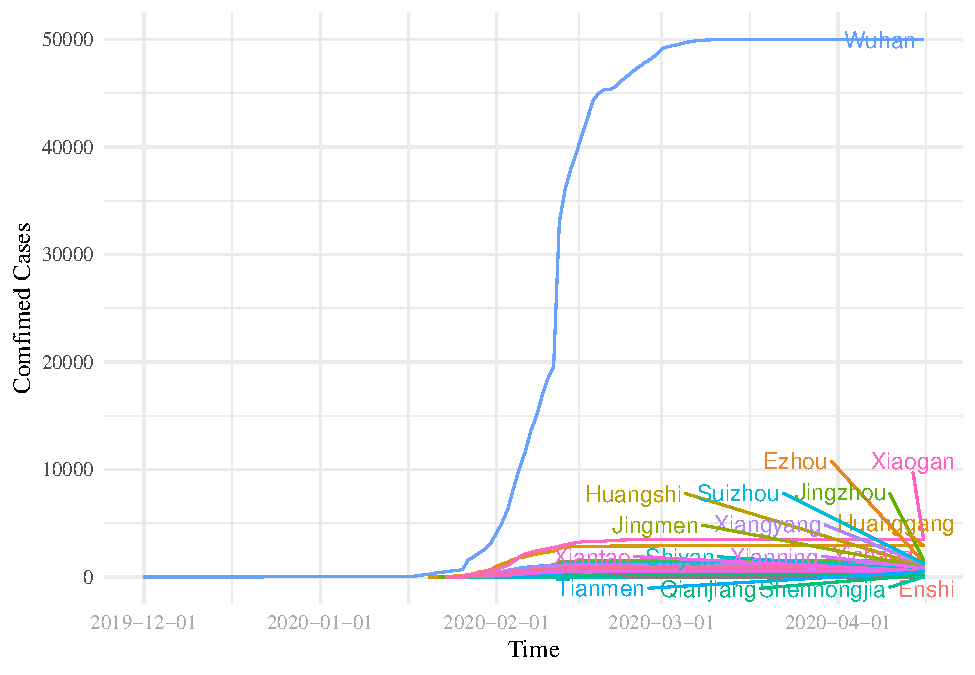
\includegraphics{Feng_ENV872_Project_files/figure-latex/HubeiCity_Trend.plot-1.pdf}
\caption{Trend of each city in Hubei province, China}
\end{figure}

\begin{quote}
Due to the confimred cases in Hubei are almost 80\% of total confimred
cases in China. I draw the trend plots for total confimred cases in
China and in each Hubei city, which shows the pattern are very similar
between Wuhan trend and China Trend.
\end{quote}

\hypertarget{trend-of-confirmed-cases-in-hubei-cities-china-except-wuhan}{%
\subsubsection{Trend of confirmed cases in Hubei cities, China (except
Wuhan)}\label{trend-of-confirmed-cases-in-hubei-cities-china-except-wuhan}}

\begin{quote}
Most cases are from Wuhan, so I deleted data from Wuhan City, and see
the if the other cities have same patterns.
\end{quote}

\begin{Shaded}
\begin{Highlighting}[]
\CommentTok{# Group by Hubei cities}
\NormalTok{Historical_HubeiCityV3 <-}\StringTok{ }\NormalTok{Historical_HubeiCityV2 }\OperatorTok
\StringTok{  }\KeywordTok{filter}\NormalTok{(city}\OperatorTok{!=}\StringTok{ "Location TBD"} \OperatorTok{&}\StringTok{ }\NormalTok{city}\OperatorTok{!=}\StringTok{ "Wuhan"}\NormalTok{) }

\CommentTok{# Save as csv}
\KeywordTok{write.csv}\NormalTok{(Historical_HubeiCityV3,}
          \DataTypeTok{file =} \StringTok{"./Data/Processed/Historical_HubeiCity (except Wuhan).csv"}\NormalTok{, }\DataTypeTok{row.names=}\OtherTok{FALSE}\NormalTok{)}
\end{Highlighting}
\end{Shaded}

\begin{Shaded}
\begin{Highlighting}[]
\CommentTok{# Create a ggplot depicting cases incereasing over time}
\NormalTok{No_Wuhan.plot <-}\StringTok{ }\KeywordTok{ggplot}\NormalTok{(Historical_HubeiCityV3, }\KeywordTok{aes}\NormalTok{(}\DataTypeTok{x=}\NormalTok{time, }\DataTypeTok{y=}\NormalTok{cum_confirm, }\DataTypeTok{color=}\NormalTok{city)) }\OperatorTok{+}
\StringTok{    }\KeywordTok{geom_line}\NormalTok{(}\DataTypeTok{alpha =} \FloatTok{0.95}\NormalTok{, }\DataTypeTok{size =} \FloatTok{0.5}\NormalTok{) }\OperatorTok{+}
\StringTok{    }\KeywordTok{geom_text_repel}\NormalTok{(}\KeywordTok{aes}\NormalTok{(}\DataTypeTok{label=}\NormalTok{city),}
                    \ControlFlowTok{function}\NormalTok{(Historical_HubeiCityV3) }
\NormalTok{                      Historical_HubeiCityV3[Historical_HubeiCityV3}\OperatorTok{$}\NormalTok{time }\OperatorTok{==}\StringTok{ }\KeywordTok{as.Date}\NormalTok{(}\StringTok{"2020-04-16"}\NormalTok{),])}\OperatorTok{+}
\StringTok{    }\NormalTok{mytheme }\OperatorTok{+}
\StringTok{    }\KeywordTok{theme}\NormalTok{(}\DataTypeTok{legend.position =} \StringTok{"none"}\NormalTok{) }\OperatorTok{+}
\StringTok{    }\KeywordTok{labs}\NormalTok{(}\DataTypeTok{x=}\KeywordTok{expression}\NormalTok{(}\KeywordTok{paste}\NormalTok{(}\StringTok{"Time"}\NormalTok{))) }\OperatorTok{+}\StringTok{ }
\StringTok{    }\KeywordTok{labs}\NormalTok{(}\DataTypeTok{y=}\KeywordTok{expression}\NormalTok{(}\KeywordTok{paste}\NormalTok{(}\StringTok{"Comfimed Cases"}\NormalTok{)))}\OperatorTok{+}
\StringTok{    }\KeywordTok{labs}\NormalTok{(}\DataTypeTok{color=}\StringTok{"city"}\NormalTok{) }\OperatorTok{+}
\StringTok{    }\KeywordTok{scale_x_date}\NormalTok{(}\DataTypeTok{date_labels =} \StringTok{"%Y-%m-%d"}\NormalTok{)}

\KeywordTok{print}\NormalTok{(No_Wuhan.plot)}
\end{Highlighting}
\end{Shaded}

\begin{figure}
\centering
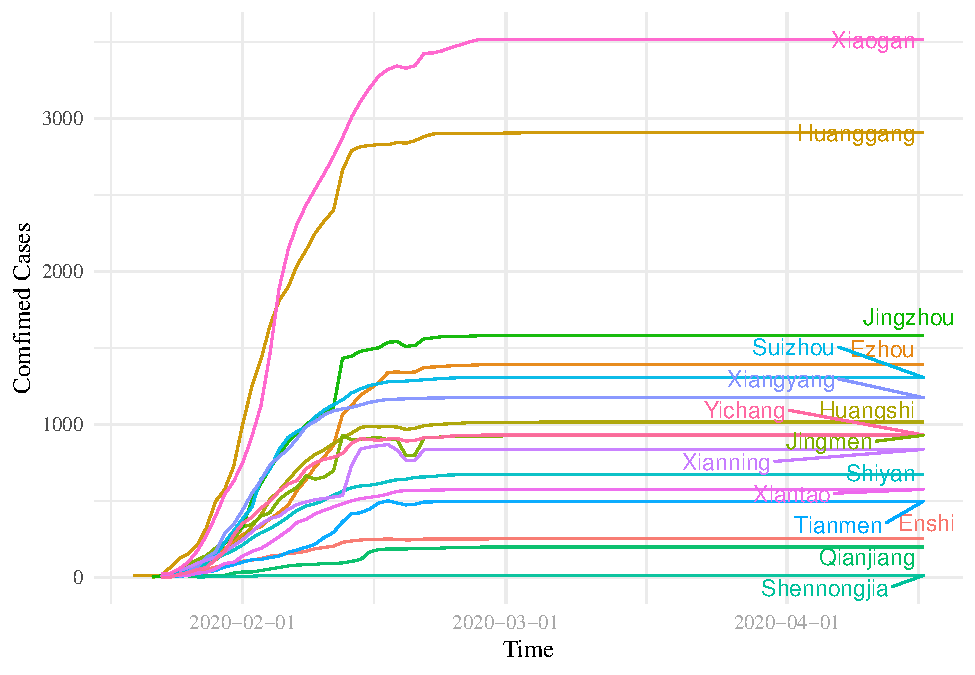
\includegraphics{Feng_ENV872_Project_files/figure-latex/No_Wuhan.plot-1.pdf}
\caption{Trend of each city in Hubei province,China (except Wuhan)}
\end{figure}

\begin{quote}
Based on the information from Wikipedia, On 23 January 2020, the central
government of China imposed a lockdown in Wuhan and other cities in
Hubei in an effort to quarantine the center of an outbreak of
coronavirus disease 2019 (COVID-19). To be noticed, Xiaogan and
Huanggang become the worst places in the country outside Wuhan, because
before the ``lockdown'' in Wuhan, the flow of people in Wuhan mainly
flowed into Xiaogan and Huanggang. Hoever, based on this action, The
confirmed cases has stabilized after one month.
\end{quote}

\hypertarget{trend-of-confirmed-cases-in-china-provincesexcept-hubei}{%
\subsubsection{Trend of confirmed cases in China provinces(except
Hubei)}\label{trend-of-confirmed-cases-in-china-provincesexcept-hubei}}

\begin{quote}
Hubei is not a typical changing pattern in China, so I deleted Hubei
data, and see patterns of other provinces.
\end{quote}

\begin{Shaded}
\begin{Highlighting}[]
\CommentTok{# Remove Hubei province data}
\NormalTok{Historical_ChinaProvince =}\StringTok{ }\NormalTok{Historical_China_processed[Historical_China_processed}\OperatorTok{$}\NormalTok{province }\OperatorTok{!=}\StringTok{ 'Hubei'}\NormalTok{,]}
\KeywordTok{head}\NormalTok{(Historical_ChinaProvince)}

\NormalTok{Historical_ChinaProvinceV2 <-}\StringTok{ }\NormalTok{Historical_ChinaProvince }\OperatorTok
\StringTok{  }\KeywordTok{group_by}\NormalTok{(time,province) }\OperatorTok
\StringTok{  }\KeywordTok{summarise}\NormalTok{(}\DataTypeTok{total_confirm =} \KeywordTok{sum}\NormalTok{(cum_confirm),}
            \DataTypeTok{total_heal =} \KeywordTok{sum}\NormalTok{(cum_heal),}
            \DataTypeTok{total_dead =} \KeywordTok{sum}\NormalTok{(cum_dead)) }

\CommentTok{# Save as csv}
\KeywordTok{write.csv}\NormalTok{(Historical_ChinaProvinceV2,}
          \DataTypeTok{file =} \StringTok{"./Data/Processed/Historical_ChinaProvince (except Hubei).csv"}\NormalTok{, }\DataTypeTok{row.names=}\OtherTok{FALSE}\NormalTok{)}
\end{Highlighting}
\end{Shaded}

\begin{Shaded}
\begin{Highlighting}[]
\CommentTok{# Create a ggplot depicting cases incereasing over time}
\NormalTok{OtherProvinces.plot <-}\StringTok{ }\KeywordTok{ggplot}\NormalTok{(Historical_ChinaProvinceV2, }\KeywordTok{aes}\NormalTok{(}\DataTypeTok{x=}\NormalTok{time, }\DataTypeTok{y=}\NormalTok{total_confirm, }\DataTypeTok{color=}\NormalTok{province)) }\OperatorTok{+}
\StringTok{    }\KeywordTok{geom_line}\NormalTok{(}\DataTypeTok{alpha =} \FloatTok{0.95}\NormalTok{, }\DataTypeTok{size =} \DecValTok{1}\NormalTok{) }\OperatorTok{+}
\StringTok{    }\KeywordTok{geom_text_repel}\NormalTok{(}\KeywordTok{aes}\NormalTok{(}\DataTypeTok{label=}\NormalTok{province),}
                    \ControlFlowTok{function}\NormalTok{(Historical_ChinaProvinceV2) }
\NormalTok{                      Historical_ChinaProvinceV2[Historical_ChinaProvinceV2}\OperatorTok{$}\NormalTok{time }\OperatorTok{==}\StringTok{ }\KeywordTok{as.Date}\NormalTok{(}\StringTok{"2020-04-16"}\NormalTok{),])}\OperatorTok{+}
\StringTok{    }\NormalTok{mytheme }\OperatorTok{+}
\StringTok{    }\KeywordTok{theme}\NormalTok{(}\DataTypeTok{legend.position =} \StringTok{"none"}\NormalTok{) }\OperatorTok{+}
\StringTok{    }\KeywordTok{labs}\NormalTok{(}\DataTypeTok{x=}\KeywordTok{expression}\NormalTok{(}\KeywordTok{paste}\NormalTok{(}\StringTok{"Time"}\NormalTok{))) }\OperatorTok{+}\StringTok{ }
\StringTok{    }\KeywordTok{labs}\NormalTok{(}\DataTypeTok{y=}\KeywordTok{expression}\NormalTok{(}\KeywordTok{paste}\NormalTok{(}\StringTok{"Comfimed Cases"}\NormalTok{))) }\OperatorTok{+}
\StringTok{    }\KeywordTok{labs}\NormalTok{(}\DataTypeTok{color=}\StringTok{"province"}\NormalTok{) }\OperatorTok{+}
\StringTok{    }\KeywordTok{scale_x_date}\NormalTok{(}\DataTypeTok{date_labels =} \StringTok{"%Y-%m-%d"}\NormalTok{)}

\KeywordTok{print}\NormalTok{(OtherProvinces.plot)}
\end{Highlighting}
\end{Shaded}

\begin{figure}
\centering
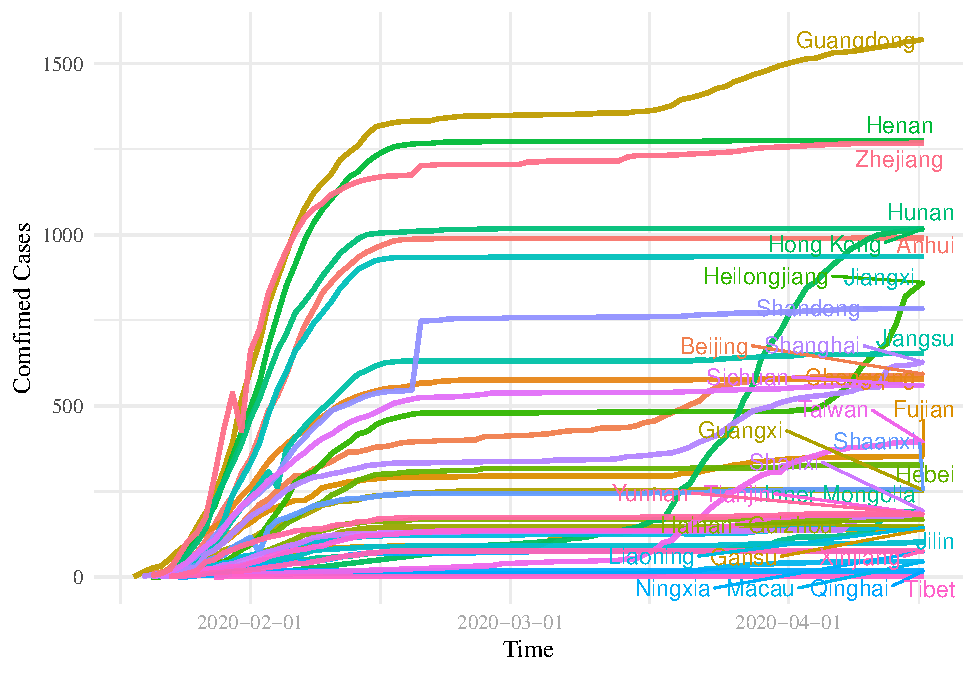
\includegraphics{Feng_ENV872_Project_files/figure-latex/OtherProvinces.plot-1.pdf}
\caption{Trend of each province in China (except Hubei)}
\end{figure}

\hypertarget{trend-of-confirmed-cases-of-top-ten-provinces-in-china-except-hubei}{%
\subsubsection{Trend of confirmed cases of top ten provinces in China
(except
Hubei)}\label{trend-of-confirmed-cases-of-top-ten-provinces-in-china-except-hubei}}

\begin{quote}
Some province are far from Hubei, and has less cases, which is also not
a typical trend pattern. Therfore, I selected top ten probince to see
their trends.
\end{quote}

\begin{Shaded}
\begin{Highlighting}[]
\CommentTok{# Filter out the top ten provinces with the highest number of diagnoses (except Hubei)}
\NormalTok{TopTen_provinces <-}\StringTok{ }\NormalTok{Historical_ChinaProvinceV2 }\OperatorTok\StringTok{ }
\StringTok{  }\KeywordTok{filter}\NormalTok{(time }\OperatorTok{>=}\StringTok{ }\KeywordTok{as.Date}\NormalTok{(}\StringTok{"2020-04-16"}\NormalTok{)) }\OperatorTok
\StringTok{  }\KeywordTok{top_n}\NormalTok{(}\DecValTok{10}\NormalTok{, total_confirm) }\OperatorTok
\StringTok{  }\KeywordTok{arrange}\NormalTok{(}\KeywordTok{desc}\NormalTok{(total_confirm)) }

\NormalTok{TopTen_provinces <-}\StringTok{ }\KeywordTok{pull}\NormalTok{(TopTen_provinces, province)}

\NormalTok{TenProvinces_China <-}\StringTok{ }\KeywordTok{filter}\NormalTok{(Historical_ChinaProvinceV2, province }\OperatorTok\StringTok{ }\NormalTok{TopTen_provinces) }\OperatorTok
\StringTok{  }\KeywordTok{arrange}\NormalTok{(}\KeywordTok{desc}\NormalTok{(total_confirm))}

\KeywordTok{head}\NormalTok{(TenProvinces_China)}

\CommentTok{# Save as csv}
\KeywordTok{write.csv}\NormalTok{(TenProvinces_China,}
          \DataTypeTok{file =} \StringTok{"./Data/Processed/TenProvinces_China (except Hubei).csv"}\NormalTok{, }\DataTypeTok{row.names=}\OtherTok{FALSE}\NormalTok{)}
\end{Highlighting}
\end{Shaded}

\begin{Shaded}
\begin{Highlighting}[]
\CommentTok{# Draw plot}
\NormalTok{TenProvinces_trend.plot <-}\StringTok{ }\KeywordTok{ggplot}\NormalTok{(TenProvinces_China, }\KeywordTok{aes}\NormalTok{(}\DataTypeTok{x =}\NormalTok{ time, }\DataTypeTok{y =}\NormalTok{total_confirm, }\DataTypeTok{color=}\NormalTok{province)) }\OperatorTok{+}
\StringTok{    }\KeywordTok{geom_line}\NormalTok{(}\DataTypeTok{alpha =} \FloatTok{0.95}\NormalTok{, }\DataTypeTok{size =} \DecValTok{1}\NormalTok{) }\OperatorTok{+}
\StringTok{    }\KeywordTok{geom_text_repel}\NormalTok{(}\KeywordTok{aes}\NormalTok{(}\DataTypeTok{label=}\NormalTok{province),}
                    \ControlFlowTok{function}\NormalTok{(Historical_ChinaProvinceV2) }
\NormalTok{                      Historical_ChinaProvinceV2[Historical_ChinaProvinceV2}\OperatorTok{$}\NormalTok{time }\OperatorTok{==}\StringTok{ }\KeywordTok{as.Date}\NormalTok{(}\StringTok{"2020-04-16"}\NormalTok{),])}\OperatorTok{+}
\StringTok{    }\NormalTok{mytheme }\OperatorTok{+}
\StringTok{    }\KeywordTok{theme}\NormalTok{(}\DataTypeTok{legend.position =} \StringTok{"none"}\NormalTok{) }\OperatorTok{+}
\StringTok{    }\KeywordTok{labs}\NormalTok{(}\DataTypeTok{x=}\KeywordTok{expression}\NormalTok{(}\KeywordTok{paste}\NormalTok{(}\StringTok{"Time"}\NormalTok{))) }\OperatorTok{+}\StringTok{ }
\StringTok{    }\KeywordTok{labs}\NormalTok{(}\DataTypeTok{y=}\KeywordTok{expression}\NormalTok{(}\KeywordTok{paste}\NormalTok{(}\StringTok{"Comfimed Cases"}\NormalTok{))) }\OperatorTok{+}
\StringTok{    }\KeywordTok{labs}\NormalTok{(}\DataTypeTok{color=}\StringTok{"province"}\NormalTok{) }\OperatorTok{+}
\StringTok{    }\KeywordTok{scale_x_date}\NormalTok{(}\DataTypeTok{date_labels =} \StringTok{"%Y-%m-%d"}\NormalTok{)}

\KeywordTok{print}\NormalTok{(TenProvinces_trend.plot)}
\end{Highlighting}
\end{Shaded}

\begin{figure}
\centering
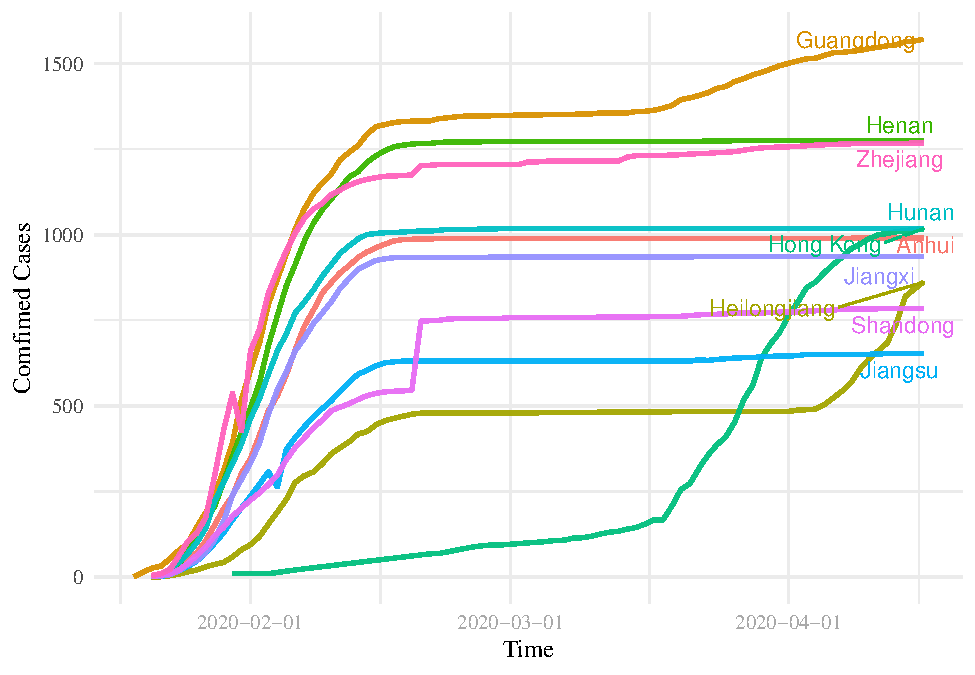
\includegraphics{Feng_ENV872_Project_files/figure-latex/TenProvinces_trend.plot-1.pdf}
\caption{Trend of top ten provinces, China (except Hubei)}
\end{figure}

\begin{quote}
Heilongjiang, Hongkong, and Guangzhou provinces should be notied form
TenProvinces\_trend.plot.
\end{quote}

\begin{quote}
According to the information I have obtained from the news, the epidemic
situation of Russia 's COVID-19 has deteriorated rapidly in the past few
days (mid-April). The number of cases of COVID-19 detected in
Helongjiang from Russia has increased, which makes it the most ``outside
import'' case in China.
\end{quote}

\begin{quote}
According to the news I saw, the reason is that the new cases in early
March were mainly from Hong Kong people who participated in two tours to
India and Egypt. The new cases increased rapidly in the second half,
mainly from people returning from overseas International students and
Hong Kong people who have settled in foreign countries, as well as the
Languifang Bar infection group.
\end{quote}

\begin{quote}
There are many people came back to Guangzhou from overseas coutries, and
cause the new increase in late March.
\end{quote}

\hypertarget{anlysis-global-trend-of-confirmed-cases-of-top-ten-countries-except-china}{%
\subsection{Anlysis Global trend of confirmed cases of top ten countries
(except
China)}\label{anlysis-global-trend-of-confirmed-cases-of-top-ten-countries-except-china}}

\begin{quote}
The breakout time of China is different from that of other countries, so
I deleted China data and see other countries patterns. Also, I selected
top ten countries to narrow down the data
\end{quote}

\begin{Shaded}
\begin{Highlighting}[]
\CommentTok{# Remove China data}
\NormalTok{Historical_Global =}\StringTok{ }\NormalTok{Historical_Global_processed[Historical_Global_processed}\OperatorTok{$}\NormalTok{country }\OperatorTok{!=}\StringTok{ 'China'}\NormalTok{,]}
\KeywordTok{str}\NormalTok{(Historical_Global)}
\end{Highlighting}
\end{Shaded}

\begin{verbatim}
## 'data.frame':    8549 obs. of  5 variables:
##  $ time       : Date, format: "2020-01-16" "2020-01-16" ...
##  $ country    : Factor w/ 205 levels "Afghanistan",..: 96 185 96 96 96 175 96 185 175 96 ...
##  $ cum_confirm: int  1 1 1 1 1 1 1 2 1 1 ...
##  $ cum_heal   : int  1 0 1 1 1 0 1 0 0 1 ...
##  $ cum_dead   : int  0 0 0 0 0 0 0 0 0 0 ...
\end{verbatim}

\begin{Shaded}
\begin{Highlighting}[]
\CommentTok{# Filter out the top ten countries with the highest number of diagnoses (except China)}
\NormalTok{TopTen_countries <-}\StringTok{ }\NormalTok{Historical_Global }\OperatorTok\StringTok{ }
\StringTok{  }\KeywordTok{filter}\NormalTok{(time }\OperatorTok{>=}\StringTok{ }\KeywordTok{as.Date}\NormalTok{(}\StringTok{"2020-04-16"}\NormalTok{)) }\OperatorTok
\StringTok{  }\KeywordTok{top_n}\NormalTok{(}\DecValTok{10}\NormalTok{, cum_confirm) }\OperatorTok
\StringTok{  }\KeywordTok{arrange}\NormalTok{(}\KeywordTok{desc}\NormalTok{(cum_confirm)) }

\CommentTok{# Selects a column in a data frame and transforms it into a vector}
\NormalTok{TopTen_countries <-}\StringTok{ }\KeywordTok{pull}\NormalTok{(TopTen_countries, country)}

\NormalTok{Historical_TopTen <-}\StringTok{ }\KeywordTok{filter}\NormalTok{(Historical_Global, country }\OperatorTok\StringTok{ }\NormalTok{TopTen_countries) }\OperatorTok
\StringTok{  }\KeywordTok{arrange}\NormalTok{(}\KeywordTok{desc}\NormalTok{(cum_confirm))}
\KeywordTok{head}\NormalTok{(Historical_TopTen)}
\end{Highlighting}
\end{Shaded}

\begin{verbatim}
##         time       country cum_confirm cum_heal cum_dead
## 1 2020-04-16 United States      650833    52739    32707
## 2 2020-04-15 United States      614726    38879    26126
## 3 2020-04-14 United States      587815    37315    23599
## 4 2020-04-13 United States      556569    32634    22063
## 5 2020-04-12 United States      529112    30548    20549
## 6 2020-04-11 United States      503177    29191    18777
\end{verbatim}

\begin{Shaded}
\begin{Highlighting}[]
\CommentTok{# Save as csv}
\KeywordTok{write.csv}\NormalTok{(Historical_TopTen,}
          \DataTypeTok{file =} \StringTok{"./Data/Processed/TopTen_countries_trend(except China).csv"}\NormalTok{, }\DataTypeTok{row.names=}\OtherTok{FALSE}\NormalTok{)}
\end{Highlighting}
\end{Shaded}

\begin{Shaded}
\begin{Highlighting}[]
\CommentTok{# Draw plot}
\NormalTok{TopTenCountries.plot <-}\StringTok{ }\KeywordTok{ggplot}\NormalTok{(Historical_TopTen, }\KeywordTok{aes}\NormalTok{(}\DataTypeTok{x =}\NormalTok{ time, }\DataTypeTok{y =}\NormalTok{cum_confirm, }\DataTypeTok{color=}\NormalTok{country)) }\OperatorTok{+}
\StringTok{    }\KeywordTok{geom_line}\NormalTok{(}\DataTypeTok{alpha =} \FloatTok{0.95}\NormalTok{, }\DataTypeTok{size =} \DecValTok{1}\NormalTok{) }\OperatorTok{+}
\StringTok{    }\KeywordTok{geom_text_repel}\NormalTok{(}\KeywordTok{aes}\NormalTok{(}\DataTypeTok{label=}\NormalTok{country),}
                    \ControlFlowTok{function}\NormalTok{(Historical_TopTen) }
\NormalTok{                      Historical_TopTen[Historical_TopTen}\OperatorTok{$}\NormalTok{time }\OperatorTok{==}\StringTok{ }\KeywordTok{as.Date}\NormalTok{(}\StringTok{"2020-04-16"}\NormalTok{),])}\OperatorTok{+}
\StringTok{    }\NormalTok{mytheme }\OperatorTok{+}
\StringTok{    }\KeywordTok{theme}\NormalTok{(}\DataTypeTok{legend.position =} \StringTok{"none"}\NormalTok{) }\OperatorTok{+}
\StringTok{    }\KeywordTok{labs}\NormalTok{(}\DataTypeTok{x=}\KeywordTok{expression}\NormalTok{(}\KeywordTok{paste}\NormalTok{(}\StringTok{"Time"}\NormalTok{))) }\OperatorTok{+}\StringTok{ }
\StringTok{    }\KeywordTok{labs}\NormalTok{(}\DataTypeTok{y=}\KeywordTok{expression}\NormalTok{(}\KeywordTok{paste}\NormalTok{(}\StringTok{"Comfimed Cases"}\NormalTok{))) }\OperatorTok{+}
\StringTok{    }\KeywordTok{labs}\NormalTok{(}\DataTypeTok{color=}\StringTok{"Country"}\NormalTok{) }\OperatorTok{+}
\StringTok{    }\KeywordTok{scale_x_date}\NormalTok{(}\DataTypeTok{date_labels =} \StringTok{"%Y-%m-%d"}\NormalTok{)}

\KeywordTok{print}\NormalTok{(TopTenCountries.plot)}
\end{Highlighting}
\end{Shaded}

\begin{figure}
\centering
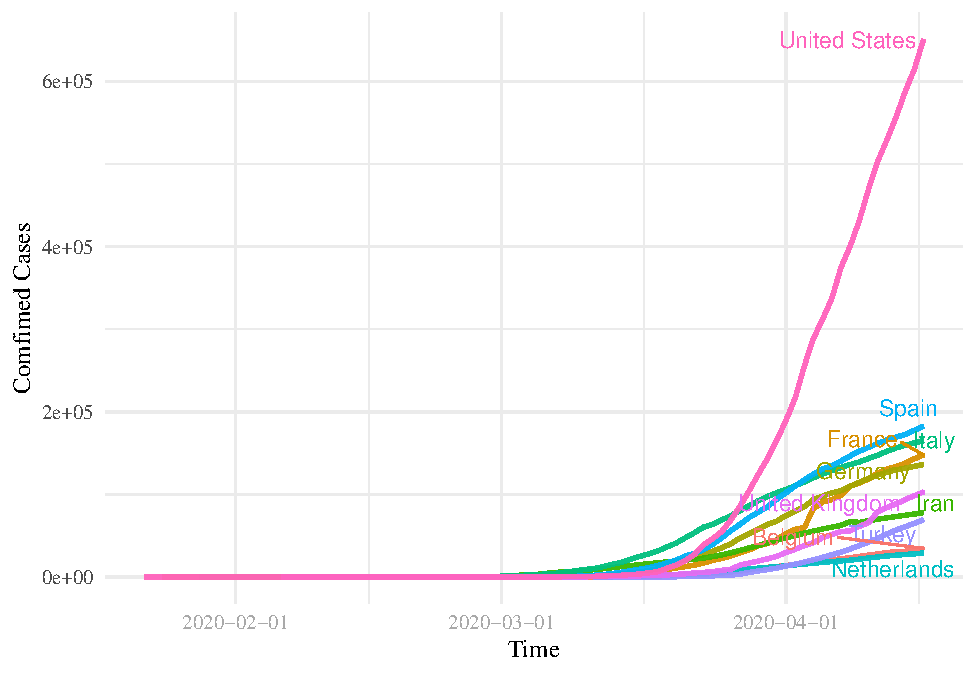
\includegraphics{Feng_ENV872_Project_files/figure-latex/TopTenCountries.plot-1.pdf}
\caption{Trend of Top Ten Countries (except China)}
\end{figure}

\hypertarget{analysis-trend-of-confirmed-cases-in-united-states.}{%
\subsection{Analysis trend of confirmed cases in United
States.}\label{analysis-trend-of-confirmed-cases-in-united-states.}}

\begin{quote}
Based on last graph, obvisiouly, the United State has the highest
confimred numbers, and I will do the analysis based on the U.S. dataset.
\end{quote}

\begin{Shaded}
\begin{Highlighting}[]
\NormalTok{Historical_USTrend <-}\StringTok{ }\NormalTok{Historical_Global_processed[Historical_Global_processed}\OperatorTok{$}\NormalTok{country }\OperatorTok{==}\StringTok{ 'United States'}\NormalTok{,] }\OperatorTok
\StringTok{  }\KeywordTok{na.omit}\NormalTok{(Historical_USTrend)}

\KeywordTok{tail}\NormalTok{(Historical_USTrend)}

\CommentTok{# Save as csv}
\KeywordTok{write.csv}\NormalTok{(Historical_USTrend,}
          \DataTypeTok{file =} \StringTok{"./Data/Processed/Historical_USTrend.csv"}\NormalTok{,}\DataTypeTok{row.names=}\OtherTok{FALSE}\NormalTok{)}
\end{Highlighting}
\end{Shaded}

\hypertarget{trend-of-total-confirmed-case-in-united-states.}{%
\subsubsection{Trend of total confirmed case in United
States.}\label{trend-of-total-confirmed-case-in-united-states.}}

\begin{quote}
First I would like to see the entire confirmed case trend through the
U.S.
\end{quote}

\begin{Shaded}
\begin{Highlighting}[]
\NormalTok{Historical_USTrend <-}\StringTok{ }\KeywordTok{read.csv}\NormalTok{(}\StringTok{"./Data/Processed/Historical_USTrend.csv"}\NormalTok{)}

\KeywordTok{head}\NormalTok{(Historical_USTrend)}
\KeywordTok{str}\NormalTok{(Historical_USTrend)}

\NormalTok{Historical_USTrend}\OperatorTok{$}\NormalTok{time <-}\StringTok{ }\KeywordTok{as.Date}\NormalTok{(Historical_USTrend}\OperatorTok{$}\NormalTok{time, }\DataTypeTok{format =} \StringTok{"%Y-%m-%d"}\NormalTok{) }
\KeywordTok{class}\NormalTok{(Historical_USTrend}\OperatorTok{$}\NormalTok{time)}
\end{Highlighting}
\end{Shaded}

\begin{Shaded}
\begin{Highlighting}[]
\NormalTok{US_Total_Trend.plot <-}
\StringTok{  }\KeywordTok{ggplot}\NormalTok{(Historical_USTrend, }\KeywordTok{aes}\NormalTok{(}\DataTypeTok{x =}\NormalTok{ time, }\DataTypeTok{y =}\NormalTok{ cum_confirm)) }\OperatorTok{+}
\StringTok{  }\KeywordTok{geom_point}\NormalTok{(}\DataTypeTok{colour =} \StringTok{"#e6550d"}\NormalTok{) }\OperatorTok{+}
\StringTok{  }\KeywordTok{geom_line}\NormalTok{(}\DataTypeTok{colour =} \StringTok{"#d95f0e"}\NormalTok{) }\OperatorTok{+}
\StringTok{  }\KeywordTok{labs}\NormalTok{(}\DataTypeTok{x =} \StringTok{"Time"}\NormalTok{, }
       \DataTypeTok{y =} \StringTok{"Confirmed Cases"}\NormalTok{) }\OperatorTok{+}\StringTok{ }
\StringTok{  }\KeywordTok{scale_x_date}\NormalTok{(}\DataTypeTok{date_labels =} \StringTok{"%Y-%m-%d"}\NormalTok{)}

\KeywordTok{print}\NormalTok{(US_Total_Trend.plot)}
\end{Highlighting}
\end{Shaded}

\begin{figure}
\centering
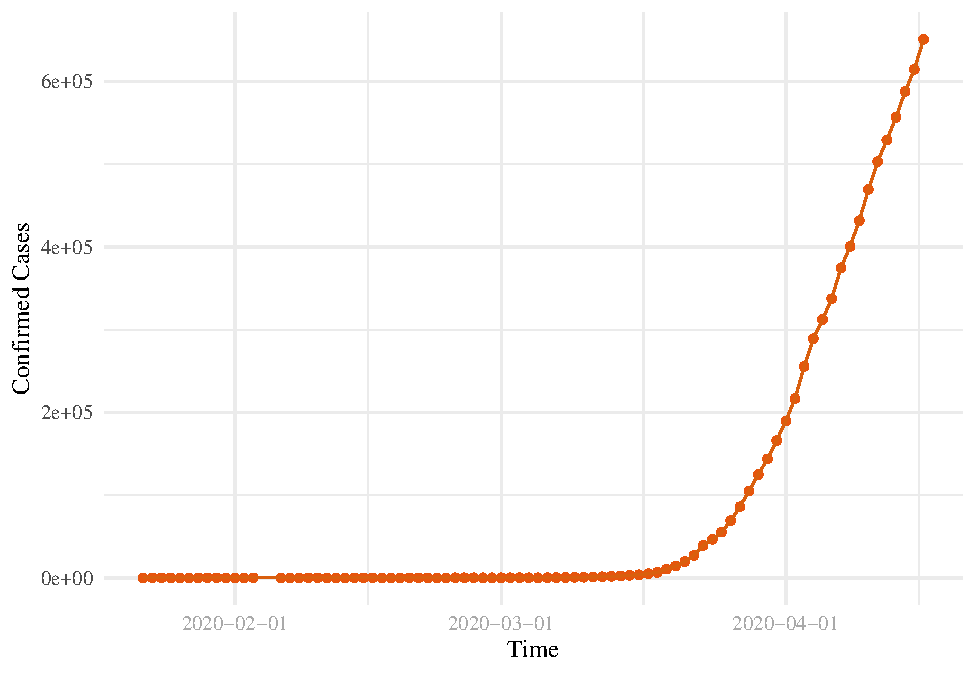
\includegraphics{Feng_ENV872_Project_files/figure-latex/US_Total_Trend.plot-1.pdf}
\caption{Trend of confirmed case in the U.S.}
\end{figure}

\hypertarget{trend-of-total-confirmed-case-in-all-states-in-the-u.s.}{%
\subsubsection{Trend of total confirmed case in all states in the
U.S.}\label{trend-of-total-confirmed-case-in-all-states-in-the-u.s.}}

\begin{Shaded}
\begin{Highlighting}[]
\CommentTok{# Create a ggplot depicting cases incereasing over time in each state}
\NormalTok{US_State_Trend.plot <-}\StringTok{ }\KeywordTok{ggplot}\NormalTok{(Covid19_US_processed, }\KeywordTok{aes}\NormalTok{(}\DataTypeTok{x=}\NormalTok{time, }\DataTypeTok{y=}\NormalTok{cum_confirm, }\DataTypeTok{color=}\NormalTok{state)) }\OperatorTok{+}
\StringTok{    }\KeywordTok{geom_line}\NormalTok{(}\DataTypeTok{alpha =} \FloatTok{0.95}\NormalTok{, }\DataTypeTok{size =} \FloatTok{0.5}\NormalTok{) }\OperatorTok{+}
\StringTok{    }\KeywordTok{geom_text_repel}\NormalTok{(}\KeywordTok{aes}\NormalTok{(}\DataTypeTok{label=}\NormalTok{state),}
                    \ControlFlowTok{function}\NormalTok{(Covid19_US_processed) }
\NormalTok{                      Covid19_US_processed[Covid19_US_processed}\OperatorTok{$}\NormalTok{time }\OperatorTok{==}\StringTok{ }\KeywordTok{as.Date}\NormalTok{(}\StringTok{"2020-04-16"}\NormalTok{),])}\OperatorTok{+}
\StringTok{    }\NormalTok{mytheme }\OperatorTok{+}
\StringTok{    }\KeywordTok{theme}\NormalTok{(}\DataTypeTok{legend.position =} \StringTok{"none"}\NormalTok{) }\OperatorTok{+}
\StringTok{    }\KeywordTok{labs}\NormalTok{(}\DataTypeTok{x=}\KeywordTok{expression}\NormalTok{(}\KeywordTok{paste}\NormalTok{(}\StringTok{"Time"}\NormalTok{))) }\OperatorTok{+}\StringTok{ }
\StringTok{    }\KeywordTok{labs}\NormalTok{(}\DataTypeTok{y=}\KeywordTok{expression}\NormalTok{(}\KeywordTok{paste}\NormalTok{(}\StringTok{"Comfimed Cases"}\NormalTok{)))}\OperatorTok{+}
\StringTok{    }\KeywordTok{labs}\NormalTok{(}\DataTypeTok{color=}\StringTok{"Covid19_US_processed"}\NormalTok{) }\OperatorTok{+}
\StringTok{    }\KeywordTok{scale_x_date}\NormalTok{(}\DataTypeTok{date_labels =} \StringTok{"%Y-%m-%d"}\NormalTok{) }

\KeywordTok{print}\NormalTok{(US_State_Trend.plot)}
\end{Highlighting}
\end{Shaded}

\begin{figure}
\centering
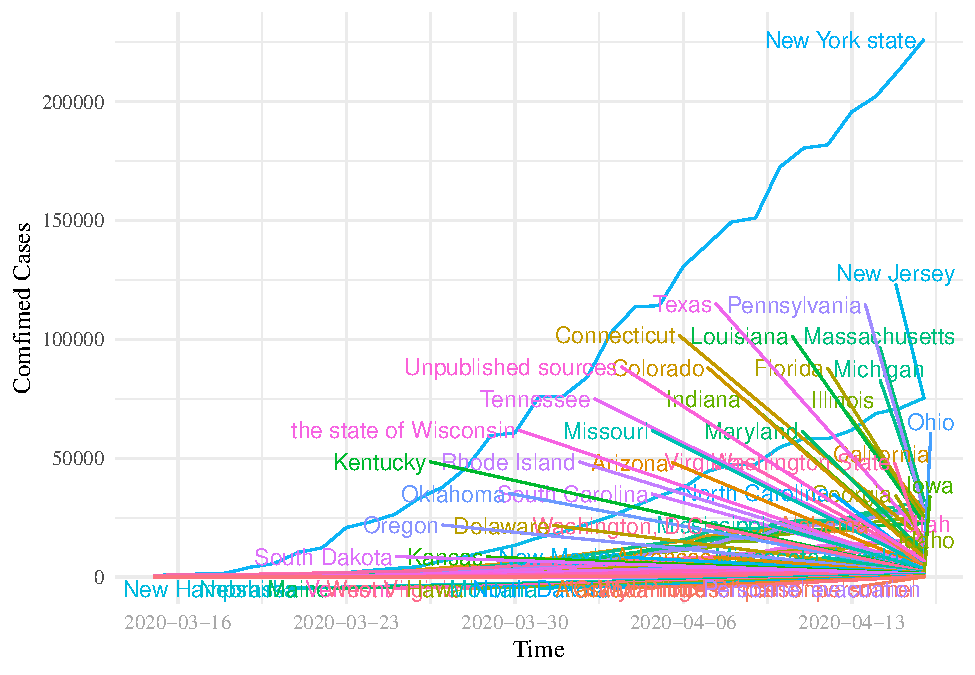
\includegraphics{Feng_ENV872_Project_files/figure-latex/US_State_Trend.plot-1.pdf}
\caption{Trend of each states in United States}
\end{figure}

\begin{quote}
I found pattern of New York is simaliar to that of whole US pattern.
\end{quote}

\hypertarget{trend-of-total-confirmed-case-of-top-ten-states-in-the-u.s.-except-ny-and-nj}{%
\subsubsection{Trend of total confirmed case of top ten states in the
U.S. (except NY and
NJ)}\label{trend-of-total-confirmed-case-of-top-ten-states-in-the-u.s.-except-ny-and-nj}}

\begin{quote}
New York and New Jersey have the almost 50\% confirmed cases in US, so I
seleted data fro these two states, and ckeck other states pattern. I
also selected top ten states, which is more representative.
\end{quote}

\begin{Shaded}
\begin{Highlighting}[]
\NormalTok{TopTen_States <-}\StringTok{ }\NormalTok{Covid19_US_processed }\OperatorTok
\StringTok{  }\KeywordTok{filter}\NormalTok{(time }\OperatorTok{>=}\StringTok{ }\KeywordTok{as.Date}\NormalTok{(}\StringTok{"2020-04-16"}\NormalTok{)) }\OperatorTok
\StringTok{  }\KeywordTok{filter}\NormalTok{(state}\OperatorTok{!=}\StringTok{ "New York state"} \OperatorTok{&}\StringTok{ }\NormalTok{state}\OperatorTok{!=}\StringTok{ "New Jersey"} \OperatorTok{&}\StringTok{ }\NormalTok{state}\OperatorTok{!=}\StringTok{ "Unpublishedsources"}\NormalTok{) }\OperatorTok
\StringTok{  }\KeywordTok{top_n}\NormalTok{(}\DecValTok{10}\NormalTok{, cum_confirm) }\OperatorTok
\StringTok{  }\KeywordTok{arrange}\NormalTok{(}\KeywordTok{desc}\NormalTok{(cum_confirm))}

\NormalTok{TopTen_States <-}\StringTok{ }\KeywordTok{pull}\NormalTok{(TopTen_States, state)}

\NormalTok{TenStates_US <-}\StringTok{ }\NormalTok{Covid19_US_processed }\OperatorTok\StringTok{ }
\StringTok{  }\KeywordTok{filter}\NormalTok{(state }\OperatorTok\StringTok{ }\NormalTok{TopTen_States) }

\KeywordTok{head}\NormalTok{(TenStates_US)}

\CommentTok{# Save as csv}
\KeywordTok{write.csv}\NormalTok{(TenStates_US,}
          \DataTypeTok{file =} \StringTok{"./Data/Processed/TenStates_US (except NY and NJ).csv"}\NormalTok{)}
\end{Highlighting}
\end{Shaded}

\begin{Shaded}
\begin{Highlighting}[]
\CommentTok{# Create a ggplot }
\NormalTok{TenStates_Trend.plot <-}\StringTok{ }\KeywordTok{ggplot}\NormalTok{(TenStates_US, }\KeywordTok{aes}\NormalTok{(}\DataTypeTok{x =}\NormalTok{ time, }\DataTypeTok{y =}\NormalTok{cum_confirm, }\DataTypeTok{color=}\NormalTok{state)) }\OperatorTok{+}
\StringTok{  }\KeywordTok{geom_line}\NormalTok{(}\DataTypeTok{alpha =} \FloatTok{0.95}\NormalTok{, }\DataTypeTok{size =} \DecValTok{1}\NormalTok{) }\OperatorTok{+}
\StringTok{  }\KeywordTok{geom_text_repel}\NormalTok{(}\KeywordTok{aes}\NormalTok{(}\DataTypeTok{label=}\NormalTok{state),}
                      \ControlFlowTok{function}\NormalTok{(TenStates_US) }
\NormalTok{                      TenStates_US[TenStates_US}\OperatorTok{$}\NormalTok{time }\OperatorTok{==}\StringTok{ }\KeywordTok{as.Date}\NormalTok{(}\StringTok{"2020-04-16"}\NormalTok{),])}\OperatorTok{+}
\StringTok{  }\NormalTok{mytheme }\OperatorTok{+}
\StringTok{  }\KeywordTok{theme}\NormalTok{(}\DataTypeTok{legend.position =} \StringTok{"none"}\NormalTok{) }\OperatorTok{+}
\StringTok{  }\KeywordTok{labs}\NormalTok{(}\DataTypeTok{x=}\KeywordTok{expression}\NormalTok{(}\KeywordTok{paste}\NormalTok{(}\StringTok{"Time"}\NormalTok{))) }\OperatorTok{+}\StringTok{ }
\StringTok{  }\KeywordTok{labs}\NormalTok{(}\DataTypeTok{y=}\KeywordTok{expression}\NormalTok{(}\KeywordTok{paste}\NormalTok{(}\StringTok{"Comfimed Cases"}\NormalTok{))) }\OperatorTok{+}
\StringTok{  }\KeywordTok{labs}\NormalTok{(}\DataTypeTok{color=}\StringTok{"state"}\NormalTok{) }\OperatorTok{+}
\StringTok{  }\KeywordTok{scale_x_date}\NormalTok{(}\DataTypeTok{date_labels =} \StringTok{"%Y-%m-%d"}\NormalTok{)}


\KeywordTok{print}\NormalTok{(TenStates_Trend.plot)}
\end{Highlighting}
\end{Shaded}

\begin{figure}
\centering
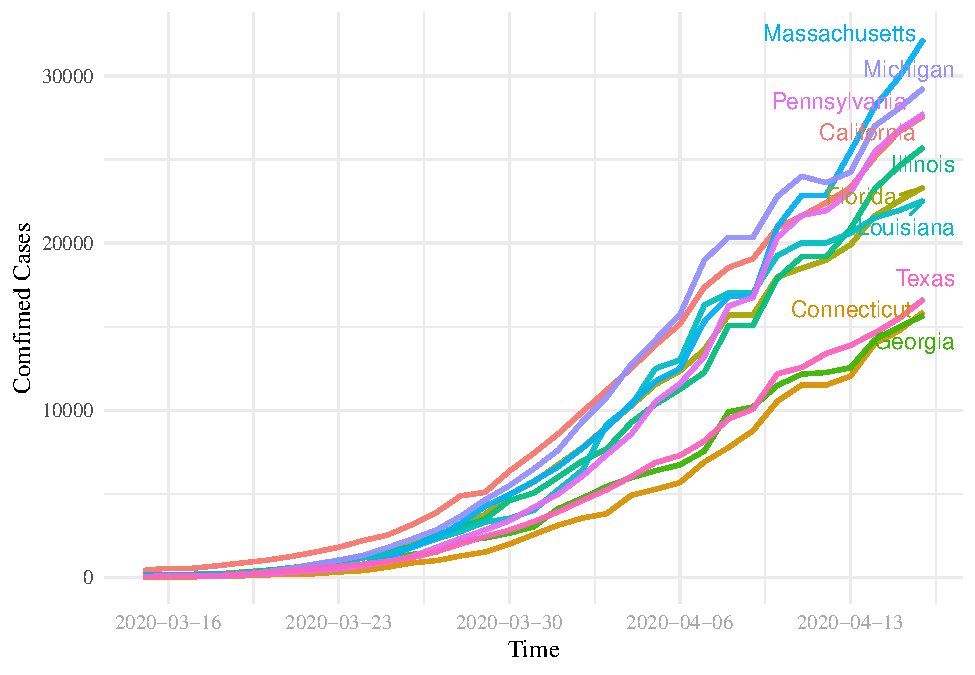
\includegraphics{Feng_ENV872_Project_files/figure-latex/TenStates_Trend.plot-1.pdf}
\caption{Trend of top ten states in United States (except NY and NJ)}
\end{figure}

\begin{quote}
Based on the top ten countries, California, Florida, Illinois, Texas and
so on, they are largest state, and has more population, which can show
it is an infectious disease.
\end{quote}

\hypertarget{analysis-trend-of-dead-and-heal-cases-number-and-rate}{%
\subsection{Analysis trend of dead and heal cases number and
rate}\label{analysis-trend-of-dead-and-heal-cases-number-and-rate}}

\hypertarget{china}{%
\subsubsection{China}\label{china}}

\begin{Shaded}
\begin{Highlighting}[]
\KeywordTok{str}\NormalTok{(Covid19_China_processed)}
\KeywordTok{head}\NormalTok{(Covid19_China_processed)}

\KeywordTok{names}\NormalTok{(Covid19_China_processed)[}\DecValTok{1}\NormalTok{] <-}\StringTok{ "Province"}
\KeywordTok{names}\NormalTok{(Covid19_China_processed)[}\DecValTok{4}\NormalTok{] <-}\StringTok{ "Dead Rate"}
\KeywordTok{names}\NormalTok{(Covid19_China_processed)[}\DecValTok{6}\NormalTok{] <-}\StringTok{ "Heal Rate"}

\NormalTok{ChinaTrend_gather <-}\StringTok{ }\NormalTok{tidyr}\OperatorTok{::}\KeywordTok{gather}\NormalTok{(Covid19_China_processed, }\StringTok{"Type"}\NormalTok{,}\StringTok{"Rate"}\NormalTok{, }\DecValTok{4}\NormalTok{,}\DecValTok{6}\NormalTok{)}
\KeywordTok{head}\NormalTok{(ChinaTrend_gather)}
\end{Highlighting}
\end{Shaded}

\begin{Shaded}
\begin{Highlighting}[]
\NormalTok{China_Rate.plot <-}\StringTok{ }\KeywordTok{ggplot}\NormalTok{(ChinaTrend_gather, }\KeywordTok{aes}\NormalTok{(}\DataTypeTok{fill=}\NormalTok{Type, }\DataTypeTok{y=}\NormalTok{Rate, }\DataTypeTok{x=}\NormalTok{Province)) }\OperatorTok{+}\StringTok{ }
\StringTok{  }\KeywordTok{geom_bar}\NormalTok{(}\DataTypeTok{stat =} \StringTok{"identity"}\NormalTok{,}\DataTypeTok{position=}\KeywordTok{position_dodge}\NormalTok{()) }\OperatorTok{+}
\StringTok{  }\KeywordTok{coord_flip}\NormalTok{() }\OperatorTok{+}
\StringTok{  }\KeywordTok{labs}\NormalTok{(}\DataTypeTok{x=}\KeywordTok{expression}\NormalTok{(}\KeywordTok{paste}\NormalTok{(}\StringTok{"Province Name"}\NormalTok{))) }\OperatorTok{+}\StringTok{ }
\StringTok{  }\KeywordTok{labs}\NormalTok{(}\DataTypeTok{y=}\KeywordTok{expression}\NormalTok{(}\KeywordTok{paste}\NormalTok{(}\StringTok{"Rate"}\NormalTok{))) }\OperatorTok{+}
\StringTok{  }\KeywordTok{labs}\NormalTok{(}\DataTypeTok{fill =} \StringTok{"Rate Types"}\NormalTok{) }\OperatorTok{+}
\StringTok{  }\NormalTok{mytheme }\OperatorTok{+}\StringTok{ }
\StringTok{  }\KeywordTok{theme}\NormalTok{(}\DataTypeTok{legend.position =} \StringTok{"right"}\NormalTok{) }
\KeywordTok{print}\NormalTok{(China_Rate.plot)}
\end{Highlighting}
\end{Shaded}

\begin{figure}
\centering
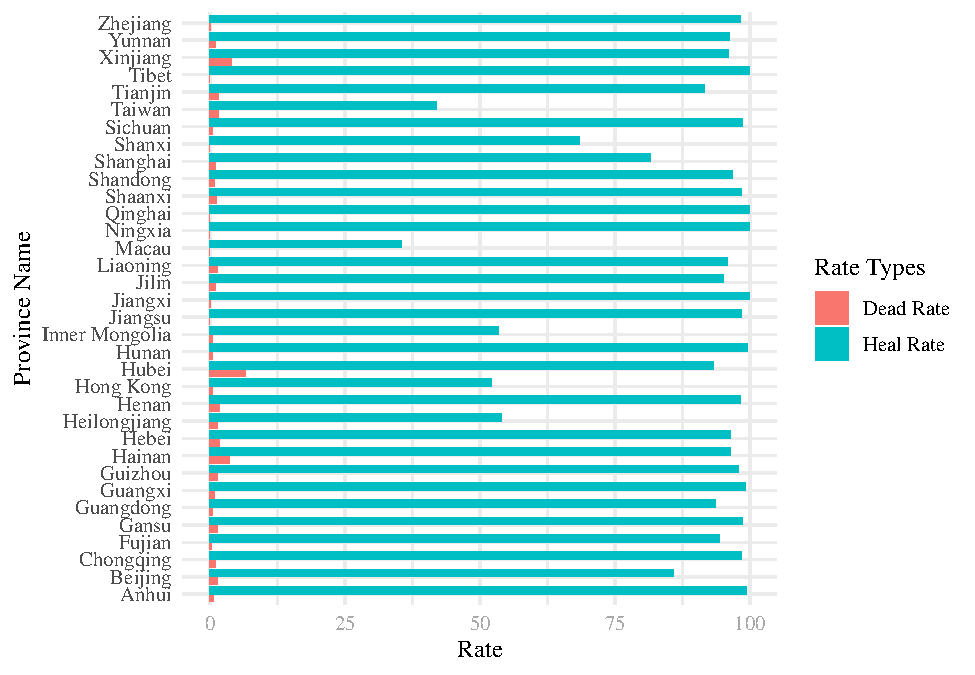
\includegraphics{Feng_ENV872_Project_files/figure-latex/China_Rate.plot-1.pdf}
\caption{Compare total death rate and heal rate in each province
(China)}
\end{figure}

\begin{quote}
In this Section, I will exeplore and analysis dead and heal cases number
and rate. I used bar plot to see the heal rate and dead rate in each
province in China (This dataset update on April 16th).
\end{quote}

\textbf{Trend of confirms, deaths,and heal number in China}

\begin{Shaded}
\begin{Highlighting}[]
\CommentTok{# Change Historical_China_processed dataset's Column names}
\KeywordTok{str}\NormalTok{(Historical_China_processed)}

\NormalTok{Historical_China_processed2 <-}\StringTok{ }\NormalTok{Historical_China_processed }\OperatorTok
\StringTok{  }\KeywordTok{group_by}\NormalTok{(time,country) }\OperatorTok
\StringTok{  }\KeywordTok{summarise}\NormalTok{(}\DataTypeTok{total_confirm =} \KeywordTok{sum}\NormalTok{(cum_confirm),}
            \DataTypeTok{total_heal =} \KeywordTok{sum}\NormalTok{(cum_heal),}
            \DataTypeTok{total_dead =} \KeywordTok{sum}\NormalTok{(cum_dead))}
\KeywordTok{head}\NormalTok{(Historical_China_processed2)}

\KeywordTok{names}\NormalTok{(Historical_China_processed2)[}\DecValTok{1}\NormalTok{] <-}\StringTok{ "Time"}
\KeywordTok{names}\NormalTok{(Historical_China_processed2)[}\DecValTok{3}\NormalTok{] <-}\StringTok{ "Total Confirm"}
\KeywordTok{names}\NormalTok{(Historical_China_processed2)[}\DecValTok{4}\NormalTok{] <-}\StringTok{ "Total Heal"}
\KeywordTok{names}\NormalTok{(Historical_China_processed2)[}\DecValTok{5}\NormalTok{] <-}\StringTok{ "Total Dead"}

\NormalTok{Historical_China_gather <-}\StringTok{ }\NormalTok{tidyr}\OperatorTok{::}\KeywordTok{gather}\NormalTok{(Historical_China_processed2, }\StringTok{"Type"}\NormalTok{, }\StringTok{"Number"}\NormalTok{, }\DecValTok{3}\OperatorTok{:}\DecValTok{5}\NormalTok{)}
\KeywordTok{str}\NormalTok{(Historical_China_gather)}
\end{Highlighting}
\end{Shaded}

\begin{Shaded}
\begin{Highlighting}[]
\NormalTok{China_Number_Trend.plot <-}\StringTok{ }\KeywordTok{ggplot}\NormalTok{(Historical_China_gather, }\KeywordTok{aes}\NormalTok{(Time, Number, }\DataTypeTok{color =}\NormalTok{ Type)) }\OperatorTok{+}
\StringTok{  }\KeywordTok{geom_point}\NormalTok{() }\OperatorTok{+}\StringTok{ }
\StringTok{  }\KeywordTok{geom_line}\NormalTok{() }\OperatorTok{+}\StringTok{ }
\StringTok{  }\KeywordTok{labs}\NormalTok{(}\DataTypeTok{x=}\KeywordTok{expression}\NormalTok{(}\KeywordTok{paste}\NormalTok{(}\StringTok{"Time"}\NormalTok{))) }\OperatorTok{+}\StringTok{ }
\StringTok{  }\KeywordTok{labs}\NormalTok{(}\DataTypeTok{y=}\KeywordTok{expression}\NormalTok{(}\KeywordTok{paste}\NormalTok{(}\StringTok{"Total number"}\NormalTok{)))}\OperatorTok{+}
\StringTok{  }\NormalTok{mytheme }\OperatorTok{+}\StringTok{ }
\StringTok{  }\KeywordTok{theme}\NormalTok{(}\DataTypeTok{legend.position =} \StringTok{"right"}\NormalTok{) }\OperatorTok{+}
\StringTok{  }\KeywordTok{scale_x_date}\NormalTok{(}\DataTypeTok{date_labels =} \StringTok{"%Y-%m-%d"}\NormalTok{)  }
\KeywordTok{print}\NormalTok{(China_Number_Trend.plot)}
\end{Highlighting}
\end{Shaded}

\begin{figure}
\centering
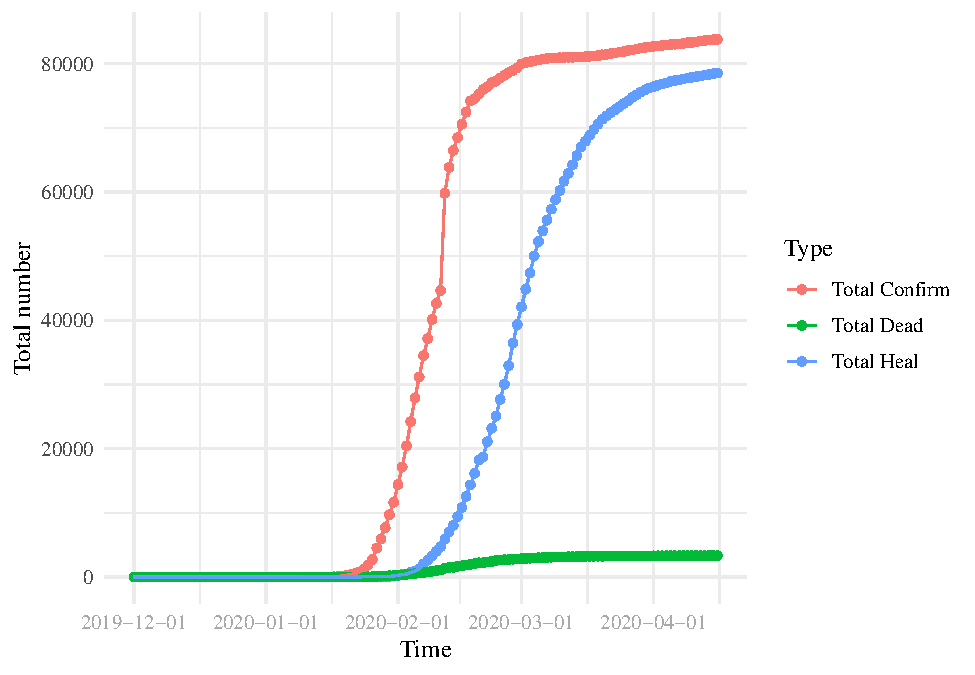
\includegraphics{Feng_ENV872_Project_files/figure-latex/China_Number_Trend.plot-1.pdf}
\caption{Trend of deaths, confirms, and heal number in China}
\end{figure}

\textbf{Trend of confirms, deaths,and heal number in China
(12/1/2019-2/15/2020")}

\begin{Shaded}
\begin{Highlighting}[]
\NormalTok{China_Number_Trend_Limit.plot <-}\StringTok{ }\KeywordTok{ggplot}\NormalTok{(Historical_China_gather, }\KeywordTok{aes}\NormalTok{(Time, Number, }\DataTypeTok{color =}\NormalTok{ Type)) }\OperatorTok{+}
\StringTok{  }\KeywordTok{geom_point}\NormalTok{() }\OperatorTok{+}\StringTok{ }
\StringTok{  }\KeywordTok{geom_line}\NormalTok{() }\OperatorTok{+}\StringTok{ }
\StringTok{  }\KeywordTok{labs}\NormalTok{(}\DataTypeTok{x=}\KeywordTok{expression}\NormalTok{(}\KeywordTok{paste}\NormalTok{(}\StringTok{"Time"}\NormalTok{))) }\OperatorTok{+}\StringTok{ }
\StringTok{  }\KeywordTok{labs}\NormalTok{(}\DataTypeTok{y=}\KeywordTok{expression}\NormalTok{(}\KeywordTok{paste}\NormalTok{(}\StringTok{"Total number"}\NormalTok{)))}\OperatorTok{+}
\StringTok{  }\NormalTok{mytheme }\OperatorTok{+}\StringTok{ }
\StringTok{  }\KeywordTok{theme}\NormalTok{(}\DataTypeTok{legend.position =} \StringTok{"right"}\NormalTok{) }\OperatorTok{+}
\StringTok{  }\KeywordTok{scale_x_date}\NormalTok{(}\DataTypeTok{date_labels =} \StringTok{"%Y-%m-%d"}\NormalTok{, }
    \DataTypeTok{limits =} \KeywordTok{c}\NormalTok{(}\KeywordTok{as.Date}\NormalTok{(}\StringTok{"2019-12-1"}\NormalTok{), }\KeywordTok{as.Date}\NormalTok{(}\StringTok{"2020-02-15"}\NormalTok{))) }\OperatorTok{+}
\StringTok{  }\KeywordTok{ylim}\NormalTok{(}\KeywordTok{c}\NormalTok{(}\DecValTok{0}\NormalTok{, }\DecValTok{500}\NormalTok{))  }
\KeywordTok{print}\NormalTok{(China_Number_Trend_Limit.plot)}
\end{Highlighting}
\end{Shaded}

\begin{figure}
\centering
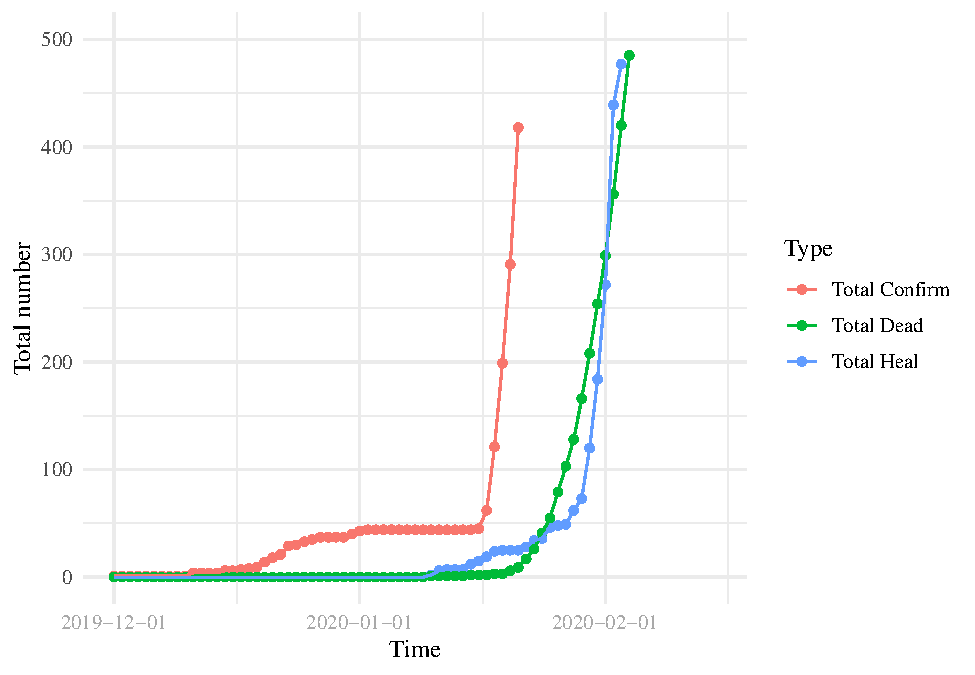
\includegraphics{Feng_ENV872_Project_files/figure-latex/China_Number_Trend_Limit.plot-1.pdf}
\caption{Trend of deaths, confirms, and heal number in China
(12/1/2019-2/15/2019}
\end{figure}

\begin{quote}
I enlarged the pattern of January and Febuary to see if there is
difference between ealry period and late period. Comparing the
trajectory of confirmed cases, heal cases, and death cases number may
have some policy experience for other countries.
\end{quote}

\begin{quote}
During the late January, the confirmed cases and death numbers are
increase rapidly. After lockdown the cities, the confirmed cases was
gruadly stablized in mid-Febuary. Therefore, the social distancing wroks
to reduece the infected cases.
\end{quote}

\textbf{Trend of confirms, deaths,and heal number top ten provines,
China}

\begin{Shaded}
\begin{Highlighting}[]
\KeywordTok{head}\NormalTok{(TenProvinces_China)}

\KeywordTok{names}\NormalTok{(TenProvinces_China)[}\DecValTok{1}\NormalTok{] <-}\StringTok{ "Time"}
\KeywordTok{names}\NormalTok{(TenProvinces_China)[}\DecValTok{3}\NormalTok{] <-}\StringTok{ "Total Confirm"}
\KeywordTok{names}\NormalTok{(TenProvinces_China)[}\DecValTok{4}\NormalTok{] <-}\StringTok{ "Total Heal"}
\KeywordTok{names}\NormalTok{(TenProvinces_China)[}\DecValTok{5}\NormalTok{] <-}\StringTok{ "Total Dead"}

\NormalTok{TenProvinces_China_gather <-}\StringTok{ }\NormalTok{tidyr}\OperatorTok{::}\KeywordTok{gather}\NormalTok{(TenProvinces_China, }\StringTok{"Type"}\NormalTok{, }\StringTok{"Number"}\NormalTok{, }\DecValTok{3}\OperatorTok{:}\DecValTok{5}\NormalTok{)}
\KeywordTok{str}\NormalTok{(TenProvinces_China_gather)}
\end{Highlighting}
\end{Shaded}

\begin{Shaded}
\begin{Highlighting}[]
\NormalTok{TenProvinces_Number_Trend.plot <-}
\StringTok{  }\KeywordTok{ggplot}\NormalTok{(TenProvinces_China_gather, }\KeywordTok{aes}\NormalTok{(}\DataTypeTok{x =}\NormalTok{ Time, }\DataTypeTok{y =}\NormalTok{ Number, }\DataTypeTok{color =}\NormalTok{ Type)) }\OperatorTok{+}
\StringTok{  }\KeywordTok{geom_line}\NormalTok{() }\OperatorTok{+}
\StringTok{  }\KeywordTok{geom_point}\NormalTok{() }\OperatorTok{+}
\StringTok{  }\KeywordTok{labs}\NormalTok{(}\DataTypeTok{x=}\KeywordTok{expression}\NormalTok{(}\KeywordTok{paste}\NormalTok{(}\StringTok{"Time"}\NormalTok{))) }\OperatorTok{+}\StringTok{ }
\StringTok{  }\KeywordTok{labs}\NormalTok{(}\DataTypeTok{y=}\KeywordTok{expression}\NormalTok{(}\KeywordTok{paste}\NormalTok{(}\StringTok{"Total number"}\NormalTok{)))}\OperatorTok{+}
\StringTok{  }\NormalTok{mytheme }\OperatorTok{+}\StringTok{ }
\StringTok{  }\KeywordTok{theme}\NormalTok{(}\DataTypeTok{legend.position =} \StringTok{"right"}\NormalTok{) }\OperatorTok{+}
\StringTok{  }\KeywordTok{scale_x_date}\NormalTok{(}\DataTypeTok{date_labels =} \StringTok{"%Y-%m-%d"}\NormalTok{, }
    \DataTypeTok{limits =} \KeywordTok{c}\NormalTok{(}\KeywordTok{as.Date}\NormalTok{(}\StringTok{"2020-1-15"}\NormalTok{), }\KeywordTok{as.Date}\NormalTok{(}\StringTok{"2020-02-15"}\NormalTok{))) }\OperatorTok{+}
\StringTok{  }\KeywordTok{ylim}\NormalTok{(}\KeywordTok{c}\NormalTok{(}\DecValTok{0}\NormalTok{, }\DecValTok{500}\NormalTok{)) }\OperatorTok{+}
\StringTok{  }\KeywordTok{facet_wrap}\NormalTok{(.}\OperatorTok{~}\NormalTok{province)}
\KeywordTok{print}\NormalTok{(TenProvinces_Number_Trend.plot)}
\end{Highlighting}
\end{Shaded}

\begin{verbatim}
## Warning: Removed 198 row(s) containing missing values (geom_path).
\end{verbatim}

\begin{verbatim}
## Warning: Removed 1909 rows containing missing values (geom_point).
\end{verbatim}

\begin{figure}
\centering
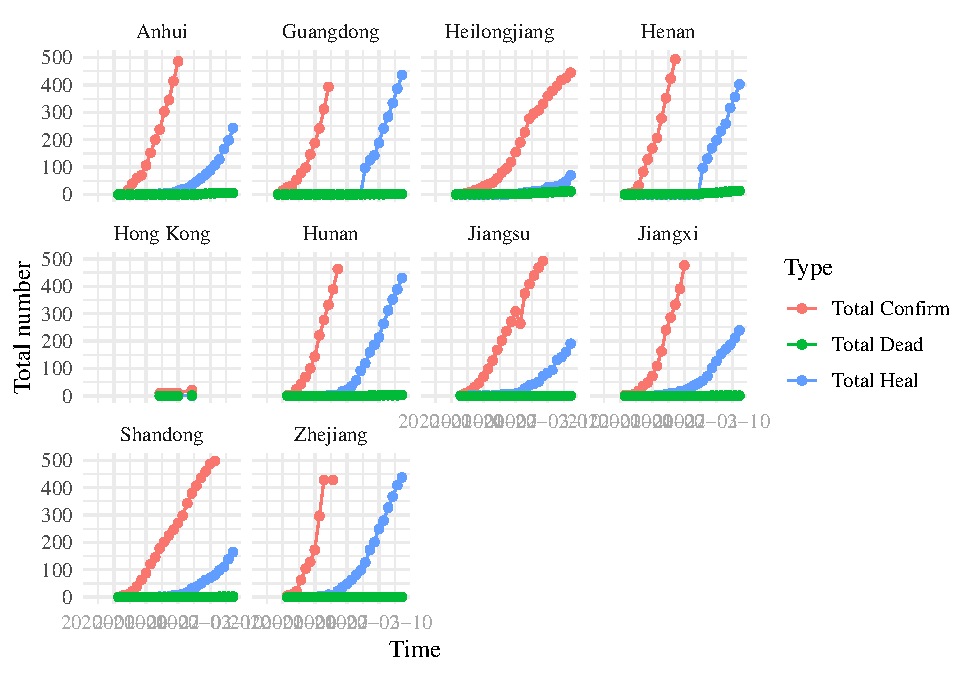
\includegraphics{Feng_ENV872_Project_files/figure-latex/TenProvinces_Number_Trend.plot (expect Hubei)-1.pdf}
\caption{Trend of deaths, confirms, and heal number in top ten provine
(expect Hubei), China}
\end{figure}

\begin{quote}
To see the trends of top ten provinces (ecpect Hubei), Guangdong, Henan,
Jiangxi, Zhejiang, and Hunan have smiliar trend. Because these five
provinces have large population movements during the Spring Festival,
and people in these province are more suspicious on COVID-19.
\end{quote}

\hypertarget{hubei-province-china}{%
\subsubsection{Hubei province, China}\label{hubei-province-china}}

\textbf{Trend of confirms, deaths,and heal number in top five cities,
Hubei(12/1/2019-3/15/2020)}

\begin{Shaded}
\begin{Highlighting}[]
\KeywordTok{head}\NormalTok{(Historical_Hubei)}

\CommentTok{# Select top five cities}
\NormalTok{TopFive_Hubei <-}\StringTok{ }\NormalTok{Historical_Hubei }\OperatorTok
\StringTok{  }\KeywordTok{filter}\NormalTok{(time }\OperatorTok{>=}\StringTok{ }\KeywordTok{as.Date}\NormalTok{(}\StringTok{"2020-04-16"}\NormalTok{)) }\OperatorTok
\StringTok{  }\KeywordTok{top_n}\NormalTok{(}\DecValTok{5}\NormalTok{, cum_confirm) }\OperatorTok
\StringTok{  }\KeywordTok{arrange}\NormalTok{(}\KeywordTok{desc}\NormalTok{(cum_confirm))}

\NormalTok{TopFive_Hubei <-}\StringTok{ }\KeywordTok{pull}\NormalTok{(TopFive_Hubei, city)}

\NormalTok{TopFiveCity_Hubei <-}\StringTok{ }\KeywordTok{filter}\NormalTok{(Historical_Hubei, city }\OperatorTok\StringTok{ }\NormalTok{TopFive_Hubei) }\OperatorTok
\StringTok{  }\KeywordTok{arrange}\NormalTok{(}\KeywordTok{desc}\NormalTok{(cum_confirm))}

\KeywordTok{head}\NormalTok{(TopFiveCity_Hubei)}

\CommentTok{# Change column names}
\KeywordTok{names}\NormalTok{(TopFiveCity_Hubei)[}\DecValTok{1}\NormalTok{] <-}\StringTok{ "Time"}
\KeywordTok{names}\NormalTok{(TopFiveCity_Hubei)[}\DecValTok{5}\NormalTok{] <-}\StringTok{ "Total Confirm"}
\KeywordTok{names}\NormalTok{(TopFiveCity_Hubei)[}\DecValTok{6}\NormalTok{] <-}\StringTok{ "Total Heal"}
\KeywordTok{names}\NormalTok{(TopFiveCity_Hubei)[}\DecValTok{7}\NormalTok{] <-}\StringTok{ "Total Dead"}

\NormalTok{Historical_Hubei_gather <-}\StringTok{ }\NormalTok{tidyr}\OperatorTok{::}\KeywordTok{gather}\NormalTok{(TopFiveCity_Hubei, }\StringTok{"Type"}\NormalTok{, }\StringTok{"Number"}\NormalTok{, }\DecValTok{5}\OperatorTok{:}\DecValTok{7}\NormalTok{)}
\KeywordTok{head}\NormalTok{(Historical_Hubei_gather)}
\end{Highlighting}
\end{Shaded}

\begin{Shaded}
\begin{Highlighting}[]
\NormalTok{FiveCities_Number_Trend.plot <-}
\StringTok{  }\KeywordTok{ggplot}\NormalTok{(Historical_Hubei_gather, }\KeywordTok{aes}\NormalTok{(}\DataTypeTok{x =}\NormalTok{ Time, }\DataTypeTok{y =}\NormalTok{ Number, }\DataTypeTok{color =}\NormalTok{ Type)) }\OperatorTok{+}
\StringTok{  }\KeywordTok{geom_line}\NormalTok{() }\OperatorTok{+}
\StringTok{  }\KeywordTok{geom_point}\NormalTok{() }\OperatorTok{+}
\StringTok{  }\KeywordTok{labs}\NormalTok{(}\DataTypeTok{x=}\KeywordTok{expression}\NormalTok{(}\KeywordTok{paste}\NormalTok{(}\StringTok{"Time"}\NormalTok{))) }\OperatorTok{+}\StringTok{ }
\StringTok{  }\KeywordTok{labs}\NormalTok{(}\DataTypeTok{y=}\KeywordTok{expression}\NormalTok{(}\KeywordTok{paste}\NormalTok{(}\StringTok{"Total number"}\NormalTok{)))}\OperatorTok{+}
\StringTok{  }\NormalTok{mytheme }\OperatorTok{+}\StringTok{ }
\StringTok{  }\KeywordTok{theme}\NormalTok{(}\DataTypeTok{legend.position =} \StringTok{"right"}\NormalTok{) }\OperatorTok{+}
\StringTok{  }\KeywordTok{scale_x_date}\NormalTok{(}\DataTypeTok{date_labels =} \StringTok{"%Y-%m-%d"}\NormalTok{, }
    \DataTypeTok{limits =} \KeywordTok{c}\NormalTok{(}\KeywordTok{as.Date}\NormalTok{(}\StringTok{"2019-12-1"}\NormalTok{), }\KeywordTok{as.Date}\NormalTok{(}\StringTok{"2020-03-15"}\NormalTok{))) }\OperatorTok{+}
\StringTok{  }\KeywordTok{ylim}\NormalTok{(}\KeywordTok{c}\NormalTok{(}\DecValTok{0}\NormalTok{, }\DecValTok{5000}\NormalTok{)) }\OperatorTok{+}
\StringTok{  }\KeywordTok{facet_wrap}\NormalTok{(.}\OperatorTok{~}\NormalTok{city)}
\KeywordTok{print}\NormalTok{(FiveCities_Number_Trend.plot)}
\end{Highlighting}
\end{Shaded}

\begin{figure}
\centering
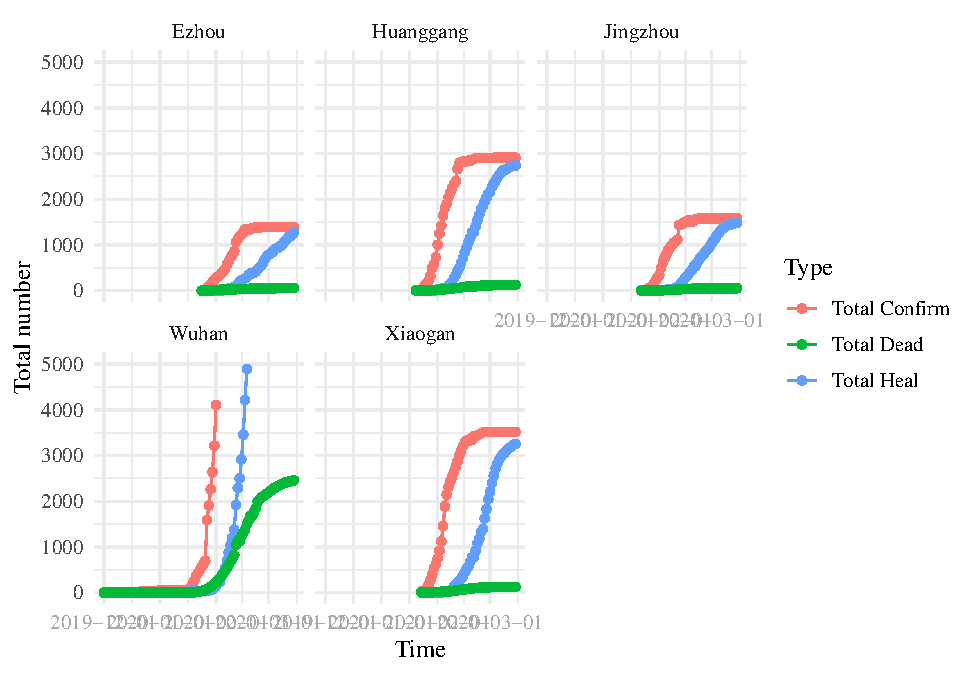
\includegraphics{Feng_ENV872_Project_files/figure-latex/FiveCities_Number_Trend.plot-1.pdf}
\caption{Trend of confirms, deaths,and heal number in top five cities,
Hubei(12/1/2019-3/15/2020)}
\end{figure}

\begin{quote}
I also pulled the top five five cities in Hubei, and found excepy Wuhan,
other cities have the same trend pattern.
\end{quote}

\hypertarget{united-states}{%
\subsubsection{United States}\label{united-states}}

\begin{Shaded}
\begin{Highlighting}[]
\CommentTok{# Change Historical_USTrend dataset's Column names}
\KeywordTok{str}\NormalTok{(Historical_USTrend)}

\NormalTok{Historical_USTrend2 <-}\StringTok{ }\NormalTok{Historical_USTrend}
\KeywordTok{names}\NormalTok{(Historical_USTrend2)[}\DecValTok{1}\NormalTok{] <-}\StringTok{ "Time"}
\KeywordTok{names}\NormalTok{(Historical_USTrend2)[}\DecValTok{3}\NormalTok{] <-}\StringTok{ "Total Confirm"}
\KeywordTok{names}\NormalTok{(Historical_USTrend2)[}\DecValTok{4}\NormalTok{] <-}\StringTok{ "Total Heal"}
\KeywordTok{names}\NormalTok{(Historical_USTrend2)[}\DecValTok{5}\NormalTok{] <-}\StringTok{ "Total Dead"}

\NormalTok{USTrend_gather <-}\StringTok{ }\NormalTok{tidyr}\OperatorTok{::}\KeywordTok{gather}\NormalTok{(Historical_USTrend2, }\StringTok{"Type"}\NormalTok{, }\StringTok{"Number"}\NormalTok{, }\DecValTok{3}\OperatorTok{:}\DecValTok{5}\NormalTok{)}
\KeywordTok{str}\NormalTok{(USTrend_gather)}
\end{Highlighting}
\end{Shaded}

\begin{Shaded}
\begin{Highlighting}[]
\NormalTok{US_Number_Trend.plot <-}\StringTok{ }\KeywordTok{ggplot}\NormalTok{(USTrend_gather, }\KeywordTok{aes}\NormalTok{(Time, Number, }\DataTypeTok{color =}\NormalTok{ Type)) }\OperatorTok{+}
\StringTok{  }\KeywordTok{geom_point}\NormalTok{() }\OperatorTok{+}\StringTok{ }
\StringTok{  }\KeywordTok{geom_line}\NormalTok{() }\OperatorTok{+}\StringTok{ }
\StringTok{  }\KeywordTok{labs}\NormalTok{(}\DataTypeTok{x=}\KeywordTok{expression}\NormalTok{(}\KeywordTok{paste}\NormalTok{(}\StringTok{"Time"}\NormalTok{))) }\OperatorTok{+}\StringTok{ }
\StringTok{  }\KeywordTok{labs}\NormalTok{(}\DataTypeTok{y=}\KeywordTok{expression}\NormalTok{(}\KeywordTok{paste}\NormalTok{(}\StringTok{"Total number"}\NormalTok{)))}\OperatorTok{+}
\StringTok{  }\NormalTok{mytheme }\OperatorTok{+}\StringTok{ }
\StringTok{  }\KeywordTok{theme}\NormalTok{(}\DataTypeTok{legend.position =} \StringTok{"right"}\NormalTok{) }\OperatorTok{+}
\StringTok{  }\KeywordTok{scale_x_date}\NormalTok{(}\DataTypeTok{date_labels =} \StringTok{"%Y-%m-%d"}\NormalTok{, }
    \DataTypeTok{limits =} \KeywordTok{c}\NormalTok{(}\KeywordTok{as.Date}\NormalTok{(}\StringTok{"2020-01-15"}\NormalTok{), }\KeywordTok{as.Date}\NormalTok{(}\StringTok{"2020-04-16"}\NormalTok{))) }
\KeywordTok{print}\NormalTok{(US_Number_Trend.plot)}
\end{Highlighting}
\end{Shaded}

\begin{figure}
\centering
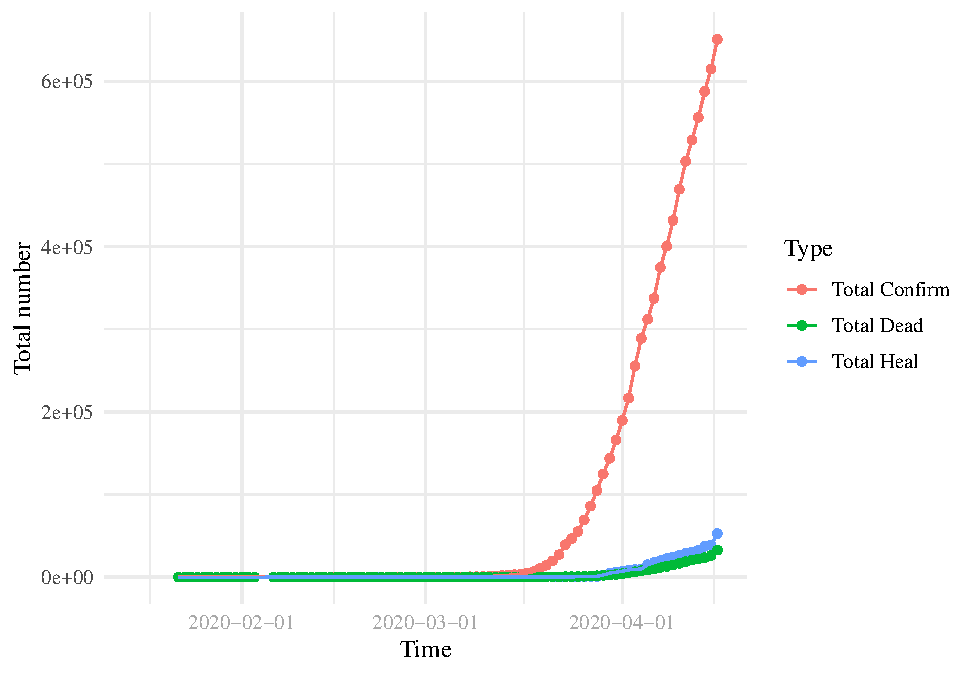
\includegraphics{Feng_ENV872_Project_files/figure-latex/US_Number_Trend.plot-1.pdf}
\caption{Trend of confirms, deaths,and heal number in the U.S.}
\end{figure}

\textbf{Heal and dead number plot for top ten states}

\begin{Shaded}
\begin{Highlighting}[]
\KeywordTok{head}\NormalTok{(TenStates_US)}

\KeywordTok{names}\NormalTok{(TenStates_US)[}\DecValTok{1}\NormalTok{] <-}\StringTok{ "Time"}
\KeywordTok{names}\NormalTok{(TenStates_US)[}\DecValTok{4}\NormalTok{] <-}\StringTok{ "Total Confirm"}
\KeywordTok{names}\NormalTok{(TenStates_US)[}\DecValTok{5}\NormalTok{] <-}\StringTok{ "Total Heal"}
\KeywordTok{names}\NormalTok{(TenStates_US)[}\DecValTok{6}\NormalTok{] <-}\StringTok{ "Total Dead"}

\NormalTok{TenStates_US_gather <-}\StringTok{ }\NormalTok{tidyr}\OperatorTok{::}\KeywordTok{gather}\NormalTok{(TenStates_US, }\StringTok{"Type"}\NormalTok{, }\StringTok{"Number"}\NormalTok{, }\DecValTok{4}\OperatorTok{:}\DecValTok{6}\NormalTok{)}
\KeywordTok{str}\NormalTok{(TenStates_US_gather)}
\end{Highlighting}
\end{Shaded}

\begin{Shaded}
\begin{Highlighting}[]
\NormalTok{Ten_States_Number_Trend.plot <-}
\StringTok{  }\KeywordTok{ggplot}\NormalTok{(TenStates_US_gather, }\KeywordTok{aes}\NormalTok{(}\DataTypeTok{x =}\NormalTok{ Time, }\DataTypeTok{y =}\NormalTok{ Number, }\DataTypeTok{color =}\NormalTok{ Type)) }\OperatorTok{+}
\StringTok{  }\KeywordTok{geom_line}\NormalTok{() }\OperatorTok{+}
\StringTok{  }\KeywordTok{geom_point}\NormalTok{() }\OperatorTok{+}
\StringTok{  }\KeywordTok{labs}\NormalTok{(}\DataTypeTok{x=}\KeywordTok{expression}\NormalTok{(}\KeywordTok{paste}\NormalTok{(}\StringTok{"Time"}\NormalTok{))) }\OperatorTok{+}\StringTok{ }
\StringTok{  }\KeywordTok{labs}\NormalTok{(}\DataTypeTok{y=}\KeywordTok{expression}\NormalTok{(}\KeywordTok{paste}\NormalTok{(}\StringTok{"Total number"}\NormalTok{)))}\OperatorTok{+}
\StringTok{  }\NormalTok{mytheme }\OperatorTok{+}\StringTok{ }
\StringTok{  }\KeywordTok{theme}\NormalTok{(}\DataTypeTok{legend.position =} \StringTok{"right"}\NormalTok{) }\OperatorTok{+}
\StringTok{  }\KeywordTok{facet_wrap}\NormalTok{(.}\OperatorTok{~}\NormalTok{state)}
\KeywordTok{print}\NormalTok{(Ten_States_Number_Trend.plot)}
\end{Highlighting}
\end{Shaded}

\begin{figure}
\centering
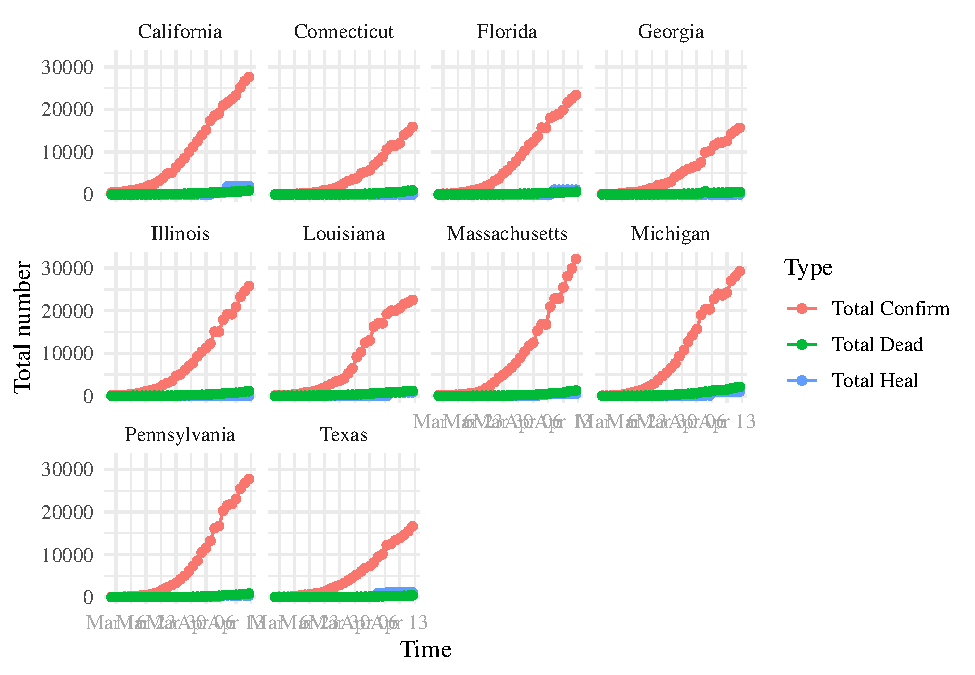
\includegraphics{Feng_ENV872_Project_files/figure-latex/Ten_States_Number_Trend.plot-1.pdf}
\caption{Trend of confirms, deaths,and heal number in top ten states}
\end{figure}

\begin{quote}
Compared tope ten states (except New York and New Jersey) to whole
United States trends. The confimred cases lines are all increasing, but
they are less steep in April than those in March.
\end{quote}

\newpage

\hypertarget{summary-and-conclusions}{%
\section{Summary and Conclusions}\label{summary-and-conclusions}}

A ``COVID-19'' epidemic caused by a new coronavirus has spread worldwide
in few months, which is an unprecedented rapid spread. China started to
lockdown cities with all countries evacuating overseas, banned
navigation, and many countries, such as United States, have closed their
borders.

This Study uses visualization method to depict incresed confirmed cases
trend on China, United States, and global level, and find their
patterns. I tried to use time series test analysis to predict the trend
of confirmeded case number, but it does not work due to short time
period. However, Hubei Province, China is the first place was reported
COVID-19. Therefore, I focus on ploting figures based on China and US
data to see if there are same patterns and relevences.

By comparing the cases trend between provinces or states and country,
contry and country, and global level, I found the intial trend pattern
are very similar. Using the trajectory of the confirmed curve and death
curve in China predicts the progress of the outbreak in the U.S. and
other countries, which is a perspective way to set up some policies.
However, the characteristics of the virus and the trend of the epidemic
are still full of variables and unknowns. Every country's actions and
every international organization's decision-making affect not only the
safety of the group's lives, but also the political and economic
development of each country, and are more likely to affect the global
situation. Therefore, even if there are similarities in early data from
various countries, one cannot assume that countries will follow the same
trajectory.

China has closed off a city of more than 11 million people in an
unprecedented effort to try to stop the spread of a deadly new virus.
Also, Everyone has a health code after stoping lockdown the cities, and
health code is an electronic voucher for individuals to pass in and out
of the local area, using the location recorded by the mobile phone GPS
to determine whether the other party is a close contact. Each state in
the U.S. also operate social-distance to prevent virvus spread. However,
China implemented restrictions earlier than other countries, and the
health code may not appear in the United States for many reasons in
western countries. Therefore, the trend of Covid-19 still need time to
tell us.

In the furture research, I will explore the relationship of Covid-19
cases number with high-risk susceptible population and race. Besides, I
would like to explore the relationship of Covid-19 with social, economic
fields, such as states GDP and states crime rate, to have a whole
overview on society and COVID-19.

\newpage

\hypertarget{references}{%
\section{References}\label{references}}

Tianzhi Wu, Erqiang Hu, Xijin Ge\emph{, Guangchuang Yu}. Open-source
analytics tools for studying the COVID-19 coronavirus outbreak. medRxiv,
2020.02.25.20027433. doi:
\url{https://doi.org/10.1101/2020.02.25.20027433}*


\end{document}
